\documentclass[11pt]{article}

% Packages
\usepackage[utf8]{inputenc}
\usepackage[T1]{fontenc}
\usepackage{amsmath, amssymb, amsfonts}
\usepackage{graphicx}
\usepackage{booktabs}
\usepackage{hyperref}
\usepackage[margin=1in]{geometry}
\usepackage{float}
\usepackage{caption}
\usepackage{subcaption}
\usepackage{multirow}
\usepackage{array}
\usepackage{tabularx}

\graphicspath{{figures/}}

\title{\textbf{Cross-Sectional Stock Return Prediction and Portfolio Construction Using Parallel Machine Learning}}
\author{
    EECE 5645 --- Parallel Processing for Data Analytics\\
    Northeastern University
}
\date{}

\begin{document}

\maketitle

\begin{abstract}
We investigate cross-sectional stock return prediction using a suite of machine learning methods implemented in a distributed computing framework. Using a panel of 499 S\&P 500 constituents observed monthly over 209 months (January 2010--November 2025) with 19 fundamental, risk, and momentum features, we compare Fama--MacBeth OLS regression, Ridge and Lasso regularization, logistic classification, stochastic gradient descent, and feedforward neural networks. All models are evaluated using expanding-window cross-validation to prevent look-ahead bias, with the Spearman Information Coefficient (IC) as the primary predictive metric and long-short decile portfolios as the economic evaluation. Ridge regression achieves the highest mean IC (0.062), while the neural network (two hidden layers, 64--32 units) achieves the best risk-adjusted portfolio performance (Sharpe ratio 2.27, maximum drawdown $-5.76\%$). All four primary models generate statistically significant Fama--French five-factor-plus-momentum alpha exceeding 27\% annualized ($t > 6.5$). We further analyze model significance via paired $t$-tests and Diebold--Mariano tests, quintile spread monotonicity, market regime resilience, signal decay, portfolio turnover and transaction costs, and feature importance across methods. All models are implemented as distributed PySpark pipelines on the Northeastern Discovery Cluster, with the neural network achieving $4.4\times$ speedup at 16 cores.
\end{abstract}

% ============================================================
\section{Introduction}
\label{sec:intro}
% ============================================================

Predicting cross-sectional stock returns is a central problem in quantitative finance. The ability to rank stocks by expected future returns enables the construction of long-short portfolios that can generate alpha independent of broad market movements. While classical approaches such as the Fama--MacBeth regression \cite{fama1973} have been used for decades, recent advances in machine learning offer the potential to capture nonlinear relationships in financial data that linear models cannot exploit.

In this paper, we apply a comprehensive suite of machine learning methods to the problem of predicting one-month-ahead stock returns using fundamental, risk, and momentum features. Our contributions are threefold. First, we implement and compare six distinct model families---OLS Fama--MacBeth, Ridge, Lasso, logistic regression, stochastic gradient descent, and neural networks---under a rigorous expanding-window evaluation framework that eliminates look-ahead bias. Second, we translate predictive signals into long-short decile portfolios and evaluate them across multiple dimensions including risk-adjusted returns, market regime resilience, transaction costs, and factor attribution. Third, we implement all models as distributed PySpark pipelines and empirically measure parallelization speedup across 1--16 cores, demonstrating how computational gains vary with per-task complexity.

\subsection{Data}

Our dataset comprises monthly observations of S\&P 500 constituent stocks sourced from the Bloomberg Terminal, spanning January 2010 through November 2025 (209 months). After filtering for data completeness, the final panel contains 93{,}237 stock-month observations across 499 unique tickers. For each stock-month, we observe 19 features organized into six categories:

\begin{itemize}
    \item \textbf{Valuation} (6): P/E ratio, price-to-sales, EV/EBITDA, price-to-free-cash-flow, dividend yield, earnings yield.
    \item \textbf{Size} (1): Market capitalization (log-transformed).
    \item \textbf{Profitability} (4): Return on assets, return on equity, gross margin, operating margin.
    \item \textbf{Leverage} (2): Total debt-to-equity, current ratio.
    \item \textbf{Risk} (3): Raw beta, 90-day realized volatility, 30-day average volume.
    \item \textbf{Technical} (3): 12-minus-1-month momentum, 3-month reversal, ratio of price to 52-week high.
\end{itemize}

The target variable is the forward one-month total return, constructed from the Bloomberg total return index (which includes dividends).

\subsection{Preprocessing}

Raw feature distributions exhibit extreme skewness and heavy tails (e.g., P/E ratio skewness of 79.8, debt-to-equity kurtosis of 7{,}330), which would distort regression estimates if left untreated. We apply three preprocessing steps cross-sectionally within each month to avoid introducing temporal information:

\begin{enumerate}
    \item \textbf{Log transformation}: Market capitalization is log-transformed to reduce right skew.
    \item \textbf{Winsorization}: Each feature is winsorized at the 1st and 99th percentiles within each month, capping extreme outliers while preserving the overall distribution shape.
    \item \textbf{Standardization}: Each feature is z-scored (mean zero, unit variance) within each month, ensuring that all features are on a comparable scale and that the cross-sectional regression coefficients are directly interpretable as effect sizes.
\end{enumerate}

The pairwise Pearson correlation matrix of the standardized features (Figure~\ref{fig:correlation}) reveals moderate collinearity among valuation ratios and among profitability metrics, with the highest pairwise correlation being 0.59 (between earnings yield and P/E ratio). This motivates the use of regularized methods (Ridge, Lasso) that can handle multicollinearity.

\begin{figure}[H]
    \centering
    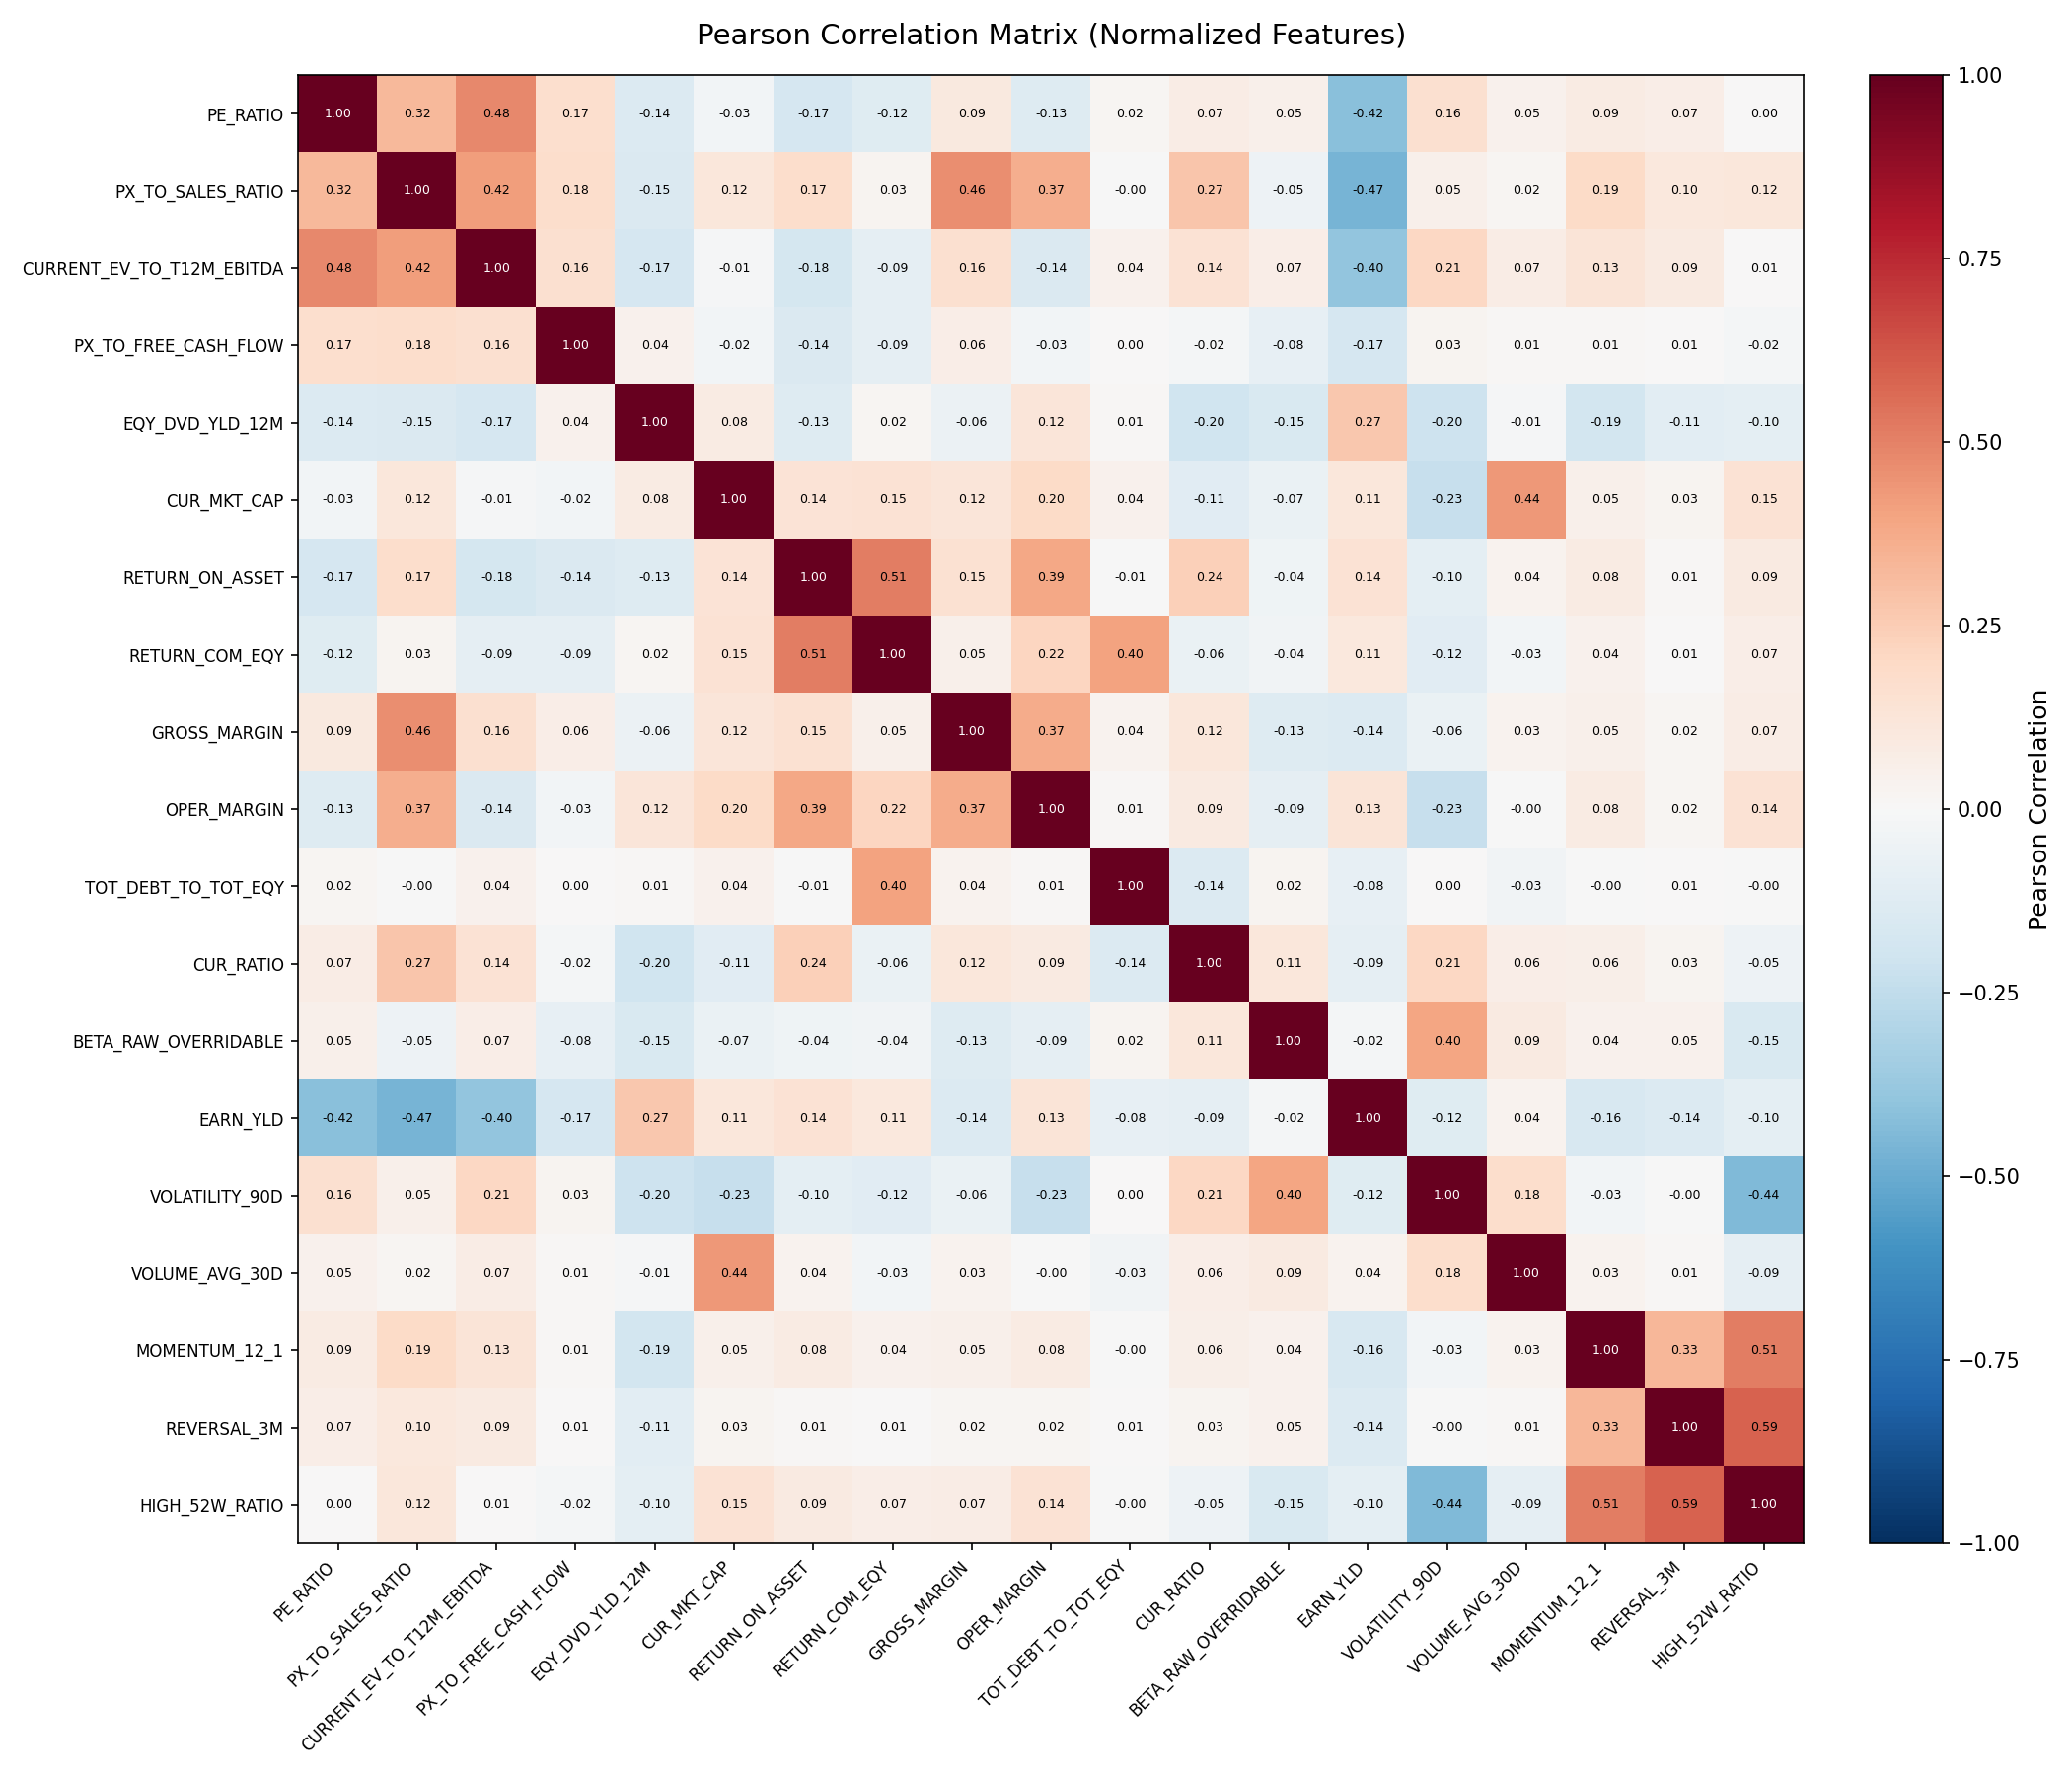
\includegraphics[width=0.85\textwidth]{correlation_heatmap.png}
    \caption{Pearson correlation matrix of the 19 standardized features, computed cross-sectionally.}
    \label{fig:correlation}
\end{figure}

\subsection{Evaluation Framework}

All models are evaluated using an expanding-window scheme with a minimum of 60 months of training data. At each month $t$ (for $t = 61, 62, \ldots, 209$), the model is trained on all observations from months $1$ through $t-1$ and generates out-of-sample predictions for month $t$. This produces 148 out-of-sample test months (approximately May 2015 through November 2025).

The primary predictive metric is the Information Coefficient (IC), defined as the Spearman rank correlation between predicted and realized returns at each month. We report the mean IC across all test months, its standard deviation, and the proportion of months with positive IC (hit rate). For economic evaluation, we construct long-short portfolios by going long the top decile and short the bottom decile of predicted returns each month, and report annualized return, annualized volatility, Sharpe ratio, and maximum drawdown.

% ============================================================
\section{Fama--MacBeth Regression}
\label{sec:fama_macbeth}
% ============================================================

We implement a Fama--MacBeth regression \cite{fama1973}, which is well-suited for data where stocks are observed over many time periods. While ridge and lasso regressions each perform a single regression on all observations from the training set, the Fama--MacBeth algorithm performs cross-sectional regressions and aggregates the results across time. However, a downside of this Fama--MacBeth implementation is that it does not use regularization like ridge and lasso regressions do. This section describes the two-step Fama--MacBeth process and the methodology for parallelizing the algorithm.

\subsection{Step 1: Cross-Sectional Regression}

First, for each time period $t$, we run a linear regression across all stocks observed at that date to estimate $r_{i,t+1}$, the return of each stock in the following period. Here, $x_{i,t}$ is the vector of features observed at time $t$ for the $i^{\text{th}}$ stock. $\alpha_t$ is the intercept, which helps account for market-wide trends. $\varepsilon_{i,t}$ is the random error component.

\begin{equation}
    y_{i,t+1} = \alpha_t + \beta_{t}^{\intercal} x_{i,t} + \varepsilon_{i,t}
\end{equation}

These cross-sectional regressions produce a separate $\beta_t$ for each time period, in contrast to standard ridge/lasso regression that fits one $\beta$ for the entire training dataset. We perform the cross-sectional linear regression using the Ordinary Least Squares (OLS) method, which is described as follows:

For a given date $t$, where $N_t$ is the number of stocks observed and $k$ is the number of features, the regression can be written using the equation

\begin{equation}
    y_t = X_t \beta_t + \varepsilon_t
\end{equation}

where $y_t \in \mathbb{R}^{N_t}$ is the vector of stock returns, $X_t \in \mathbb{R}^{N_t \times (k+1)}$ is the matrix of features (including a column of ones for the intercept), and $\beta_t \in \mathbb{R}^{k+1}$ is the vector of regression coefficients.

The OLS estimator minimizes the sum of squared error

\begin{equation}
    \min_{\beta_t} \| y_t - X_t \beta_t \|^2
\end{equation}

using the closed-form solution

\begin{equation}
    \hat{\beta}_t = (X_t^{\intercal} X_t)^{-1} X_t^{\intercal} y_t
\end{equation}

$\hat{\beta}_t$ is computed independently for each time period.

\subsection{Step 2: Aggregation Across Time}

The coefficient vector estimates are then aggregated by simply computing the time-series average, where $T$ is the number of time periods:

\begin{equation}
    \bar{\beta} = \frac{1}{T}\sum_{t=1}^{T} \hat{\beta}_t
\end{equation}

This final Fama--MacBeth estimate reflects the average relationship between the features and stock returns across all time periods of the training set.

The time-series standard errors of $\hat{\beta}_t$ provide a natural test of whether each factor commands a significant risk premium. Table~\ref{tab:factor_premia} reports the factors with the strongest premia. Market capitalization is the most significant predictor ($t = -9.13$), with the negative sign indicating that smaller stocks earn higher returns. Realized volatility ($t = 5.16$) and trading volume ($t = 4.66$) are also highly significant, consistent with the low-volatility anomaly operating in reverse at the monthly horizon and with volume serving as a proxy for liquidity or attention.

\begin{table}[H]
\centering
\caption{Fama--MacBeth factor premia: factors significant at the 1\% level across all regimes.}
\label{tab:factor_premia}
\begin{tabular}{lrrr}
\toprule
Factor & Mean Coefficient & $t$-statistic & $p$-value \\
\midrule
\verb|CUR_MKT_CAP|       & $-0.00368$ & $-9.132$ & $<0.001$ \\
\verb|VOLATILITY_90D|     & $+0.00467$ & $+5.158$ & $<0.001$ \\
\verb|VOLUME_AVG_30D|     & $+0.00207$ & $+4.655$ & $<0.001$ \\
\verb|OPER_MARGIN|        & $+0.00210$ & $+3.705$ & $<0.001$ \\
\verb|PX_TO_FREE_CASH_FLOW| & $-0.00087$ & $-2.657$ & $0.009$ \\
\verb|PX_TO_SALES_RATIO|  & $-0.00162$ & $-2.616$ & $0.010$ \\
\bottomrule
\end{tabular}
\end{table}

\subsection{Parallelized Implementation}

Because each cross-sectional regression is independent of the others, the Fama--MacBeth method can be conveniently implemented using parallel computation. We implemented the algorithm using PySpark on the Northeastern Discovery Cluster. First, the data is loaded into a Resilient Distributed Dataset (RDD), and partitioned using the \verb|Date| of each observation as the key. This ensures all observations from a given time period are located on the same worker.

The cross-sectional regression is then performed for each \verb|Date|, which does not require shuffling the RDD or passing data between workers. We implemented this by mapping each observation to $x^{\intercal}x$ and $x^{\intercal}y$, reducing by the \verb|Date| key to sum each time period's subset, then using \verb|numpy.linalg.lstsq| to compute each $\hat{\beta}_t$.

The $\hat{\beta}_t$ is then averaged across the training set to produce the final estimate. Due to the time-series nature of the data, we used expanding window cross validation to test the Fama--MacBeth implementation. The cross-sectional regressions only needed to be computed once, then for each expanding window iteration we averaged $\hat{\beta}_t$ up to a specific date and tested a prediction of the next time period's stock returns. This ensures that the model is never trained using data from the test set or future observations.

The result of the expanding window validation was a mean IC of 0.0602, with a 70.95\% hit rate over 148 test months. The portfolio backtest produced a 28.73\% annualized return with a Sharpe ratio of 2.03.

% ============================================================
\section{Ridge and Lasso Regression}
\label{sec:ridge_lasso}
% ============================================================

We used Ridge (L2) and Lasso (L1) regularized regression \cite{hoerl1970, tibshirani1996} on the same panel of stock-month observations used in the OLS Fama--MacBeth baseline. These regularized regressions are generally used to address limitations of ordinary least squares regression, such as sensitivity to multicollinearity and overfitting. Both methods alter the standard regression model with a penalty term that discourages large coefficients and controls model complexity. Ridge shrinks all coefficients towards zero but retains all features, while Lasso can shrink some coefficients to zero, effectively performing a level of factor selection.

The regularized loss function for Ridge regression takes the form:

\begin{equation}
    \hat{\beta} = \arg\min_{\beta} \sum_{i=1}^{n} (y_i - x_i^{\intercal} \beta)^2 + \lambda \|\beta\|_2^2
\end{equation}

and for Lasso:

\begin{equation}
    \hat{\beta} = \arg\min_{\beta} \sum_{i=1}^{n} (y_i - x_i^{\intercal} \beta)^2 + \lambda \|\beta\|_1
\end{equation}

where $y_i$ is the forward one-month return for stock $i$, $x_i$ is the vector of features, and $\lambda$ is the regularization parameter controlling the strength of the regularization.

Both models were trained using expanding-window evaluation rather than random $k$-fold cross-validation. This design choice is critical for financial time-series data, as using future observations to train a model that is tested on the past would create look-ahead bias and inflate performance estimates. In our setup, a minimum of 60 months of training data was required before generating the first prediction. At each subsequent time step, all available prior observations are used for training, and the model generates out-of-sample predictions for the following month. The regularization parameter $\lambda$ was selected via this same expanding-window procedure, with the optimal $\lambda$ chosen to maximize the mean Information Coefficient.

Model performance was evaluated using the Information Coefficient (IC), defined as the Spearman rank correlation between predicted and realized forward returns at each month. The IC is a standard metric in quantitative equity research because it is robust to outliers in the return distribution and directly captures whether the model correctly ranks stocks by expected return, which is the relevant objective for portfolio construction. A mean IC above zero indicates that the model has actual predictive power, while the IC's standard deviation and the proportion of months with positive IC provide insight into the consistency and reliability of predictions across the data.

\subsection{Results and Validation}

The Ridge model achieved a mean IC of 0.0623, with a standard deviation of 0.119 and a hit rate of 72.97\%. The Lasso model achieved a mean IC of 0.0512, with 6 out of 19 features receiving non-zero coefficients on average across the evaluation window. The features selected by Lasso were \verb|CUR_MKT_CAP|, \verb|OPER_MARGIN|, \verb|BETA_RAW_OVERRIDABLE|, \verb|VOLATILITY_90D|, \verb|VOLUME_AVG_30D|, and \verb|REVERSAL_3M|, suggesting that these factors carry the most reliable return signal.

The evolution of Lasso coefficients over the expanding window is shown in Figure~\ref{fig:lasso_coefficients}. The rolling IC values for both Ridge and Lasso (Figure~\ref{fig:ridge_lasso_ic}) show that Ridge and Lasso produced a similar curve shape of IC values throughout the rolling window, but Ridge regularly outperformed Lasso.

\begin{figure}[H]
    \centering
    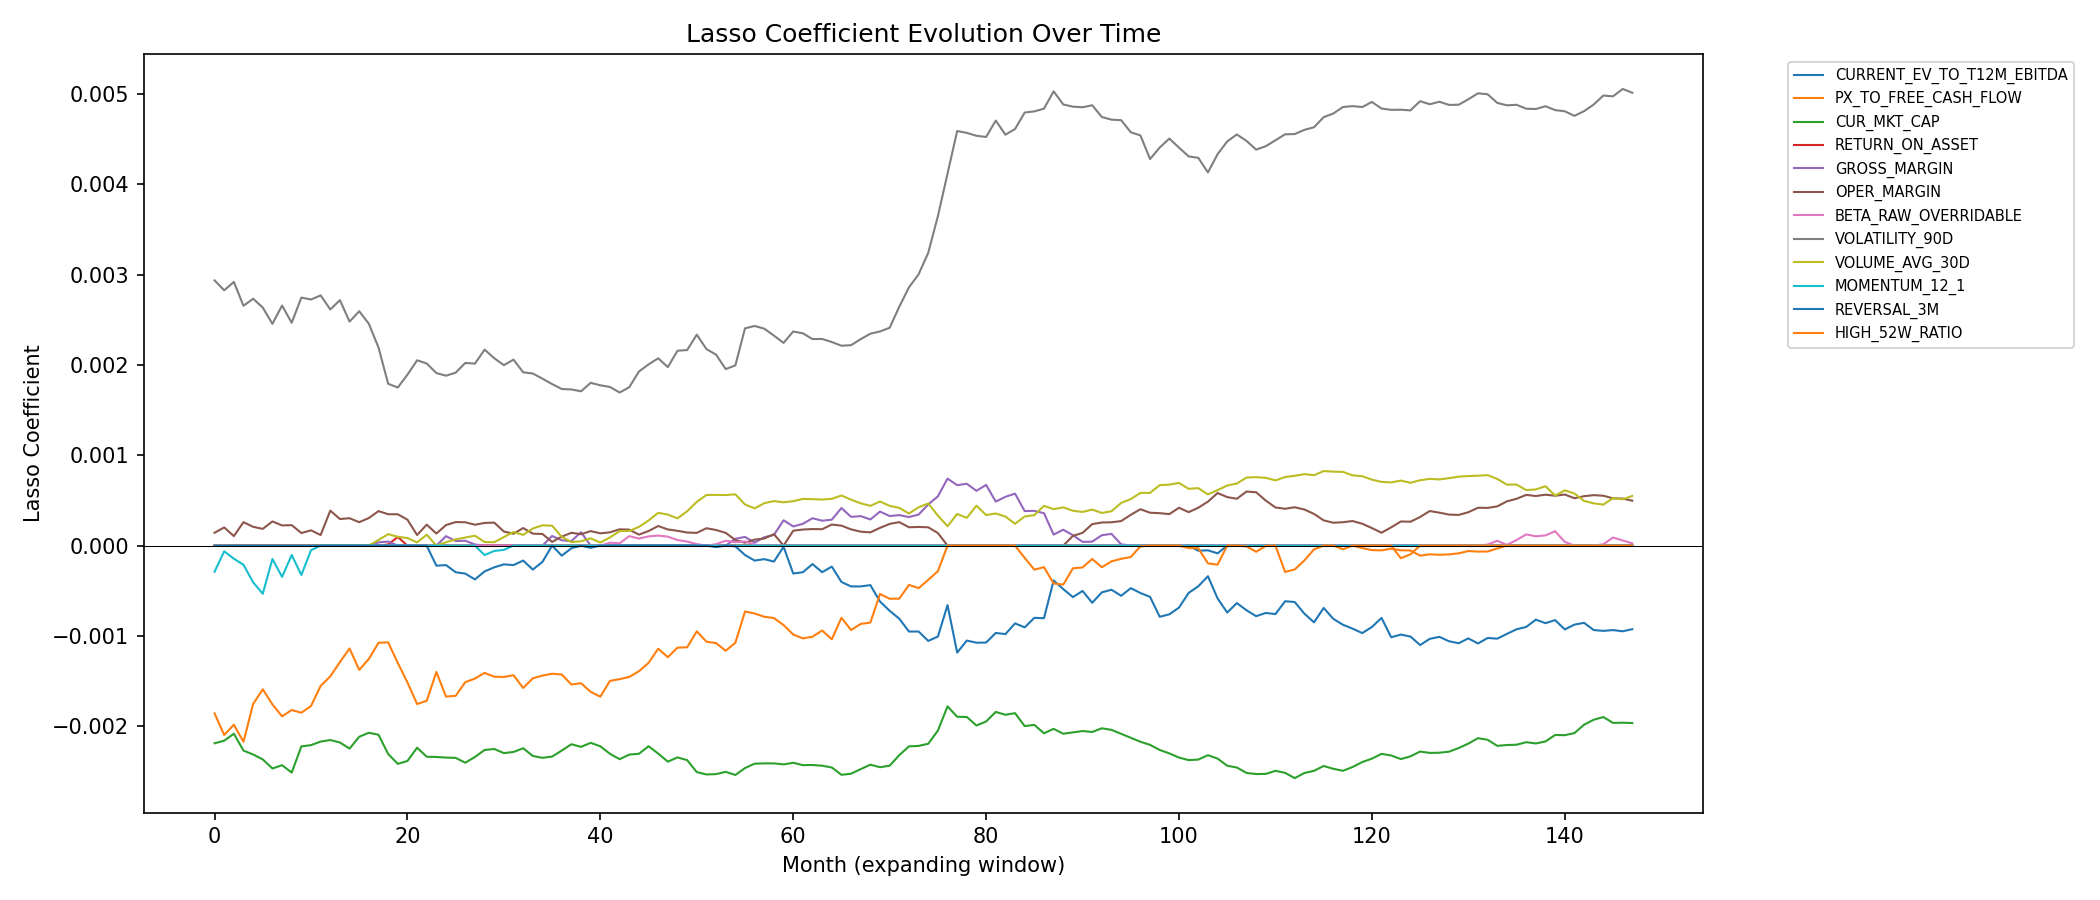
\includegraphics[width=0.8\textwidth]{lasso_coefficients.png}
    \caption{Evolution of Lasso regression coefficients over the expanding evaluation window.}
    \label{fig:lasso_coefficients}
\end{figure}

\begin{figure}[H]
    \centering
    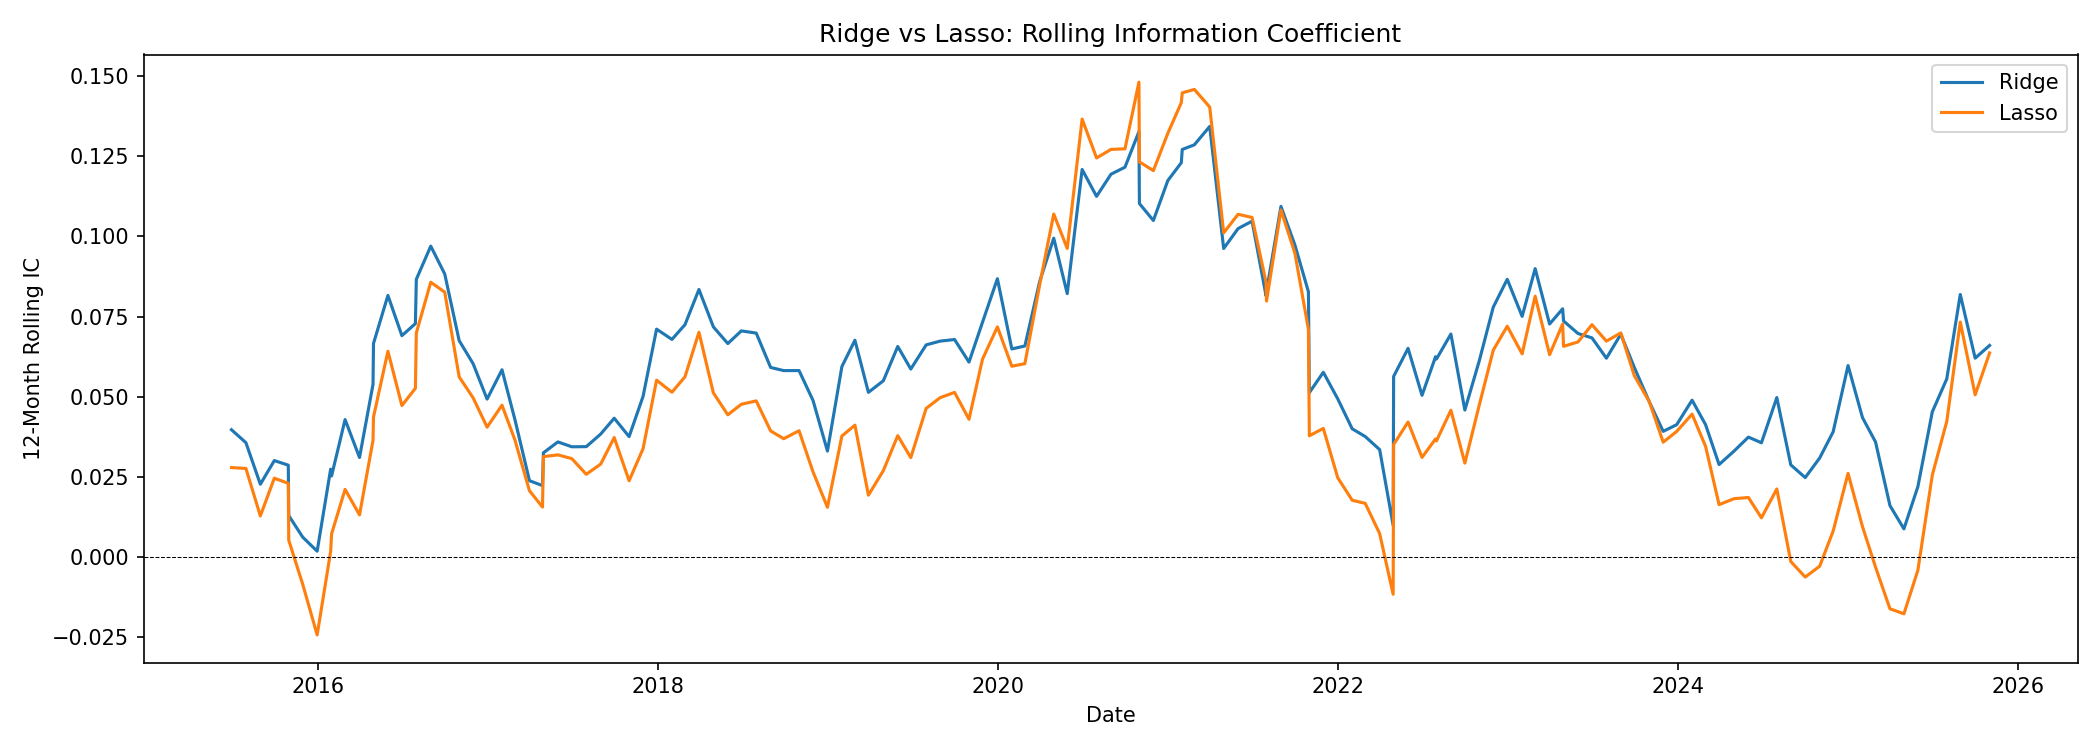
\includegraphics[width=0.8\textwidth]{ridge_vs_lasso_ic.png}
    \caption{Rolling Information Coefficient for Ridge and Lasso regression.}
    \label{fig:ridge_lasso_ic}
\end{figure}

The general consistency of the IC across time provides a strong quality signal. A mean IC of 0.0623 paired with 72.97\% positive-IC months for Ridge indicates that the model's predictive edge is not driven by a small number of lucky months but holds reliably across the majority of the evaluation period. We compared the performance of both regularized models against the unregularized OLS baseline. The fact that Ridge outperforms OLS (0.0623 vs.\ 0.0602) confirms that regularization is providing a meaningful improvement in generalization. For Lasso, the reduction in IC relative to Ridge is expected given its aggressive feature elimination. The six retained features represent a meaningful factor set spanning size, profitability, risk, and reversal, lending interpretive credibility to the solution. Taken together, the positive and consistent out-of-sample IC across both models, the improvement of Ridge over the unregularized baseline, and the economically interpretable feature selection by Lasso collectively support the conclusion that the regularized solutions are of good quality and not artifacts of overfitting.

\subsection{Parallelism}

Both Ridge and Lasso regression were trained within a distributed Spark pipeline designed to exploit the embarrassingly parallel structure of the expanding-window scheme. At each time step, the model must be fit on an independent training dataset and evaluated on a held-out test month. This is a workload that involves no data dependencies across time windows and is therefore well-suited to parallelization. The Spark implementation partitions the set of evaluation windows across available workers, with each worker independently constructing its training matrix, fitting the regularized regression via Ridge or Lasso, and returning its predictions. Hyperparameter tuning was similarly parallelized, with different values of $\lambda$ dispatched to separate workers for simultaneous evaluation.

We measured runtime for both Ridge and Lasso across a range of worker counts: 1, 2, 4, 8, and 16 cores. The speedup for each is reported relative to the single-core baseline, and the results are plotted in Figure~\ref{fig:speedup} alongside the ideal linear speedup curve for reference.

As shown in the figure, both Ridge and Lasso exhibit positive speedup as the number of cores increases, confirming that the distributed implementation successfully reduces execution time relative to sequential execution. However, the observed speedup falls well short of the ideal linear curve for both models. Ridge in particular shows very low gains, reaching a speedup of approximately $1.28\times$ at 16 cores, while Lasso achieved a more noticeable but still sub-linear speedup of approximately $2.29\times$ at 16 cores.

Ridge was fit using scikit-learn's \verb|solver='auto'| setting, which allows the library to internally select the most appropriate solver based on the data characteristics. Regardless of which solver was selected, we can see that Ridge's solution is inherently inexpensive to compute per window once the training matrix is assembled, meaning that the per-task compute time is short relative to the fixed Spark overhead of task scheduling, data serialization, and driver result aggregation. As a result, adding more cores did not substantially reduce execution time because the bottleneck is coordination rather than computation.

Lasso required iterative coordinate descent to converge and was therefore more compute-intensive per evaluation window. This higher per-task cost led to Lasso achieving a more meaningful speedup. The flattening of the Lasso speedup curve between 8 and 16 cores suggests that the pipeline approaches a point at which adding further workers yields diminishing returns, likely due to worker communication costs. The $2.29\times$ speedup at 16 cores shows a tangible benefit of the distributed implementation for the more compute-intensive model, and both models confirm the expected pattern that parallelism helps more when per-task computation is the dominant cost.

\begin{figure}[H]
    \centering
    
\includegraphics[width=0.8\textwidth]{speedup_chart.png}
    \caption{Speedup vs.\ number of cores for all four models. The dashed line indicates ideal linear speedup.}
    \label{fig:speedup}
\end{figure}

\begin{figure}[H]
    \centering
    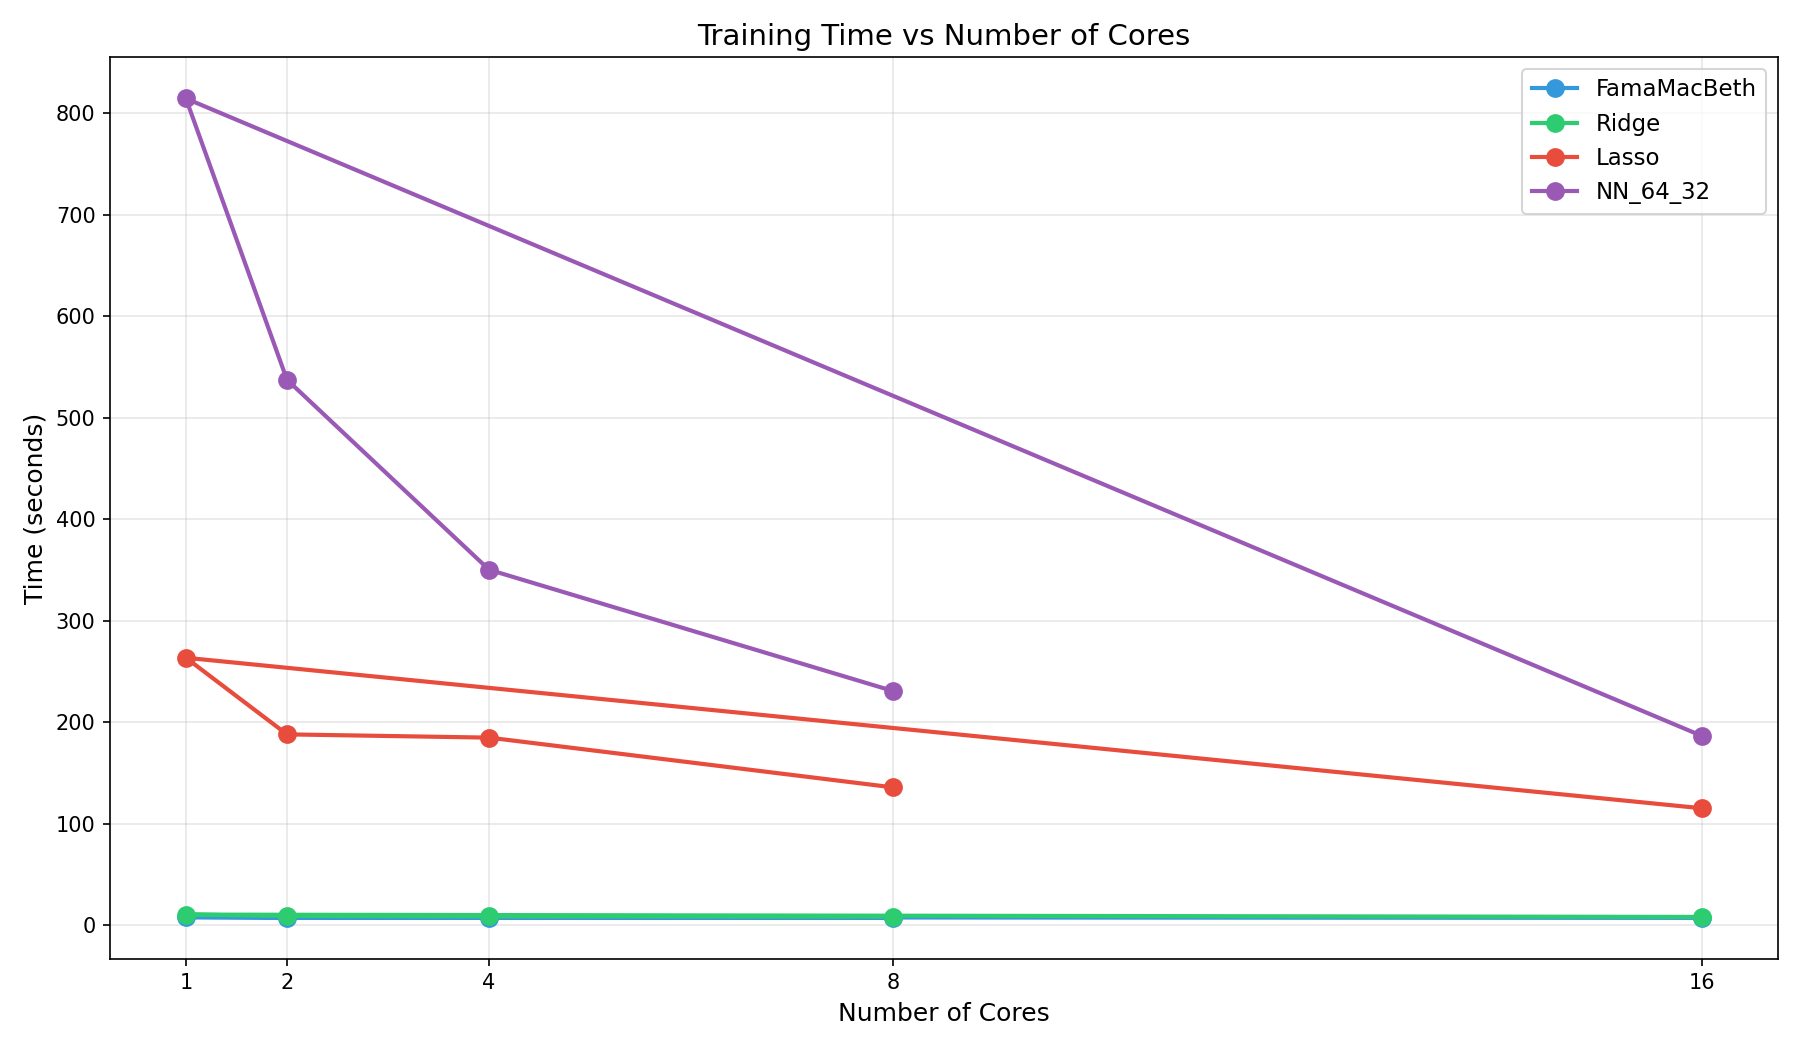
\includegraphics[width=0.8\textwidth]{time_vs_cores.png}
    \caption{Execution time vs.\ number of cores for all four models.}
    \label{fig:execution_time}
\end{figure}

% ============================================================
\section{Logistic Regression}
\label{sec:logistic}
% ============================================================

We also used binary classification for the return prediction problem. Rather than predicting the continuous forward return directly, we classified each stock-month observation as belonging to the top quintile (20\%) of returners (label = 1) or the bottom quintile (20\%) (label = 0), and discarded the middle 60\% of the return distribution from training and evaluation. This structure was motivated by the practical reality of portfolio construction, as a long-short equity strategy requires only the ability to distinguish likely outperformers from likely underperformers, not an accurate estimate of every stock's return. Excluding the middle quintiles sharpens the learning signal by ensuring that the model is trained on observations where the distinction between classes is most meaningful.

The binary labels were assigned cross-sectionally within each month, meaning labelling was done within each month separately. Logistic regression was then applied to predict the probability that a given stock belongs to the top quintile given its feature vector. The model was trained using a maximum of 10{,}000 iterations, fitting the sigmoid function:

\begin{equation}
    P(y = 1 \mid x) = \frac{1}{1 + e^{-x^{\intercal}\beta}}
\end{equation}

where $\beta$ is estimated by maximizing the log-likelihood subject to an L2 penalty controlled by the inverse regularization strength parameter $C$. $C = 1/\lambda$, so smaller values of $C$ correspond to stronger regularization. We trained with four values of $C$ (0.01, 0.1, 1.0, 10.0) to assess the classification performance sensitivity to the degree of regularization applied to the model.

As with the regression models, evaluation was performed using an expanding-window scheme with a minimum of 60 months of training data. At each test month, the model generates predicted class probabilities for each stock, and performance is measured using the Area Under the ROC Curve (AUC) and classification accuracy. AUC is the primary metric of interest because it measures the model's ability to distinguish between the top and bottom quintile. An AUC of 0.5 corresponds to a random classifier, while an AUC of 1.0 corresponds to a perfect one.

\subsection{Results and Validation}

The model produced a mean AUC of 0.544 for all values of $C$. Similarly, the mean accuracy for each value of $C$ was about 52\% over 148 evaluation months. The proportion of months with AUC $> 0.5$ was 70\%, indicating that the model maintained above-random predictive ability in the large majority of time periods. By market regime, the model showed AUC of 0.557 during Bull markets, 0.542 during Neutral conditions, and 0.338 during Crash periods. The aggregated ROC curve for the model is shown in Figure~\ref{fig:roc_curve}, along with a plot of the 12-month rolling AUC over the evaluation window in Figure~\ref{fig:rolling_auc}.

Since all values of $C$ produced an identical AUC, we can say that the model is insensitive to regularization strength. Although an AUC of 0.544 is only marginally above the random baseline of 0.5, this classification task is inherently difficult given the high noise-to-signal ratio in equity returns, and even a small edge above 0.5 can be economically meaningful.

As seen in the rolling AUC plot, AUC stays consistently above 0.5 for the entire window, peaking at about 0.58. Since the model never dips below the random baseline of 0.5, we can say that the model is consistently better than random, even if the advantage is minimal.

\begin{figure}[H]
    \centering
    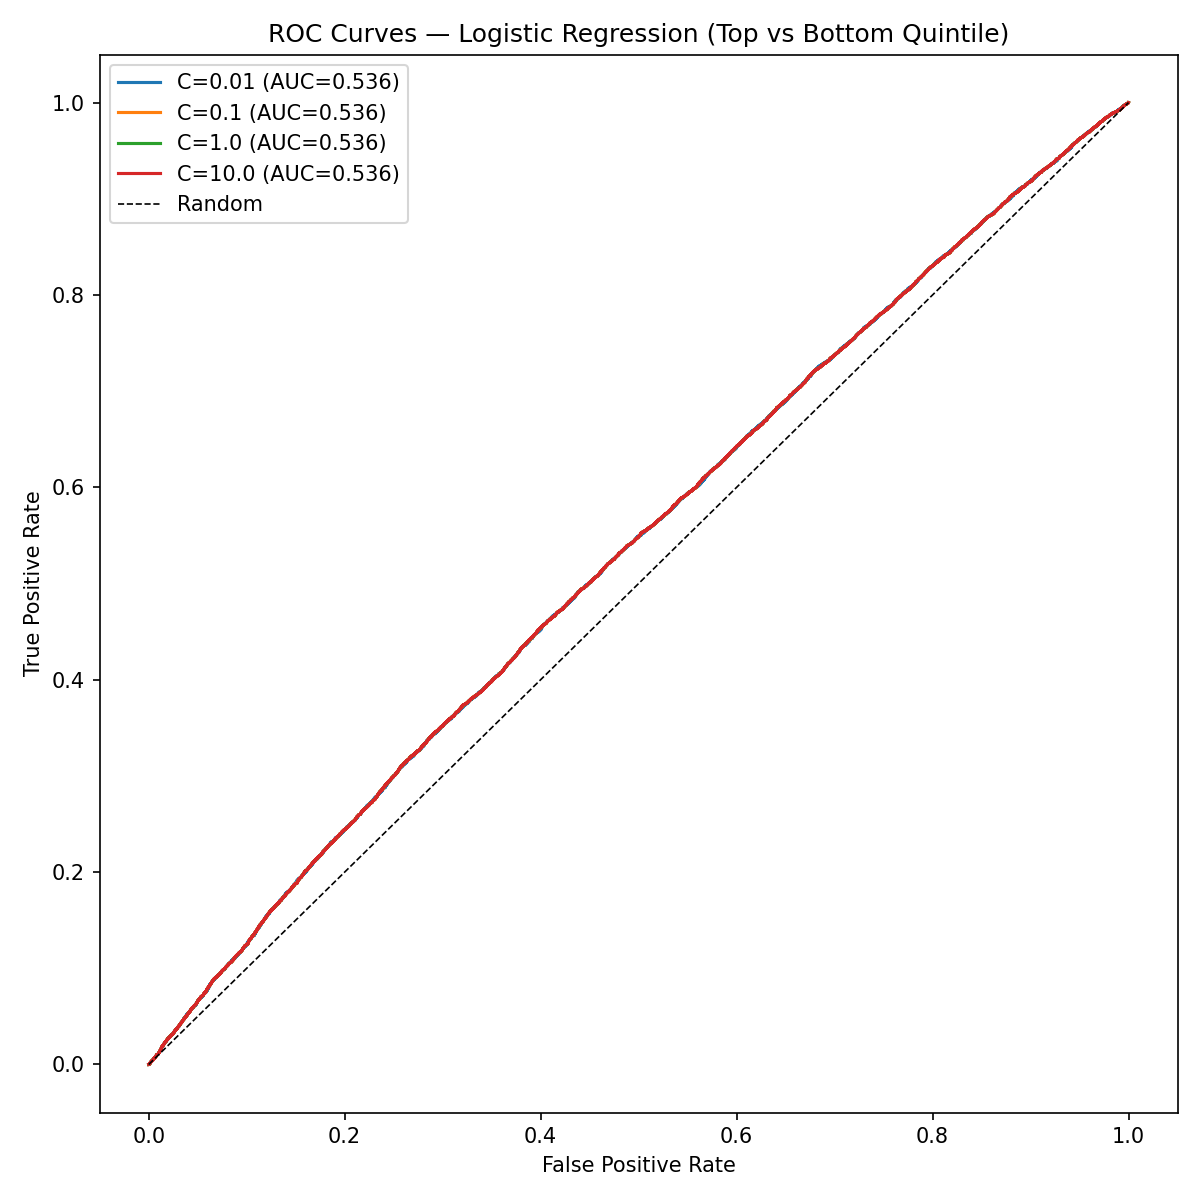
\includegraphics[width=0.7\textwidth]{roc_curves.png}
    \caption{Aggregated ROC curve for logistic regression across different values of regularization strength $C$.}
    \label{fig:roc_curve}
\end{figure}

\begin{figure}[H]
    \centering
    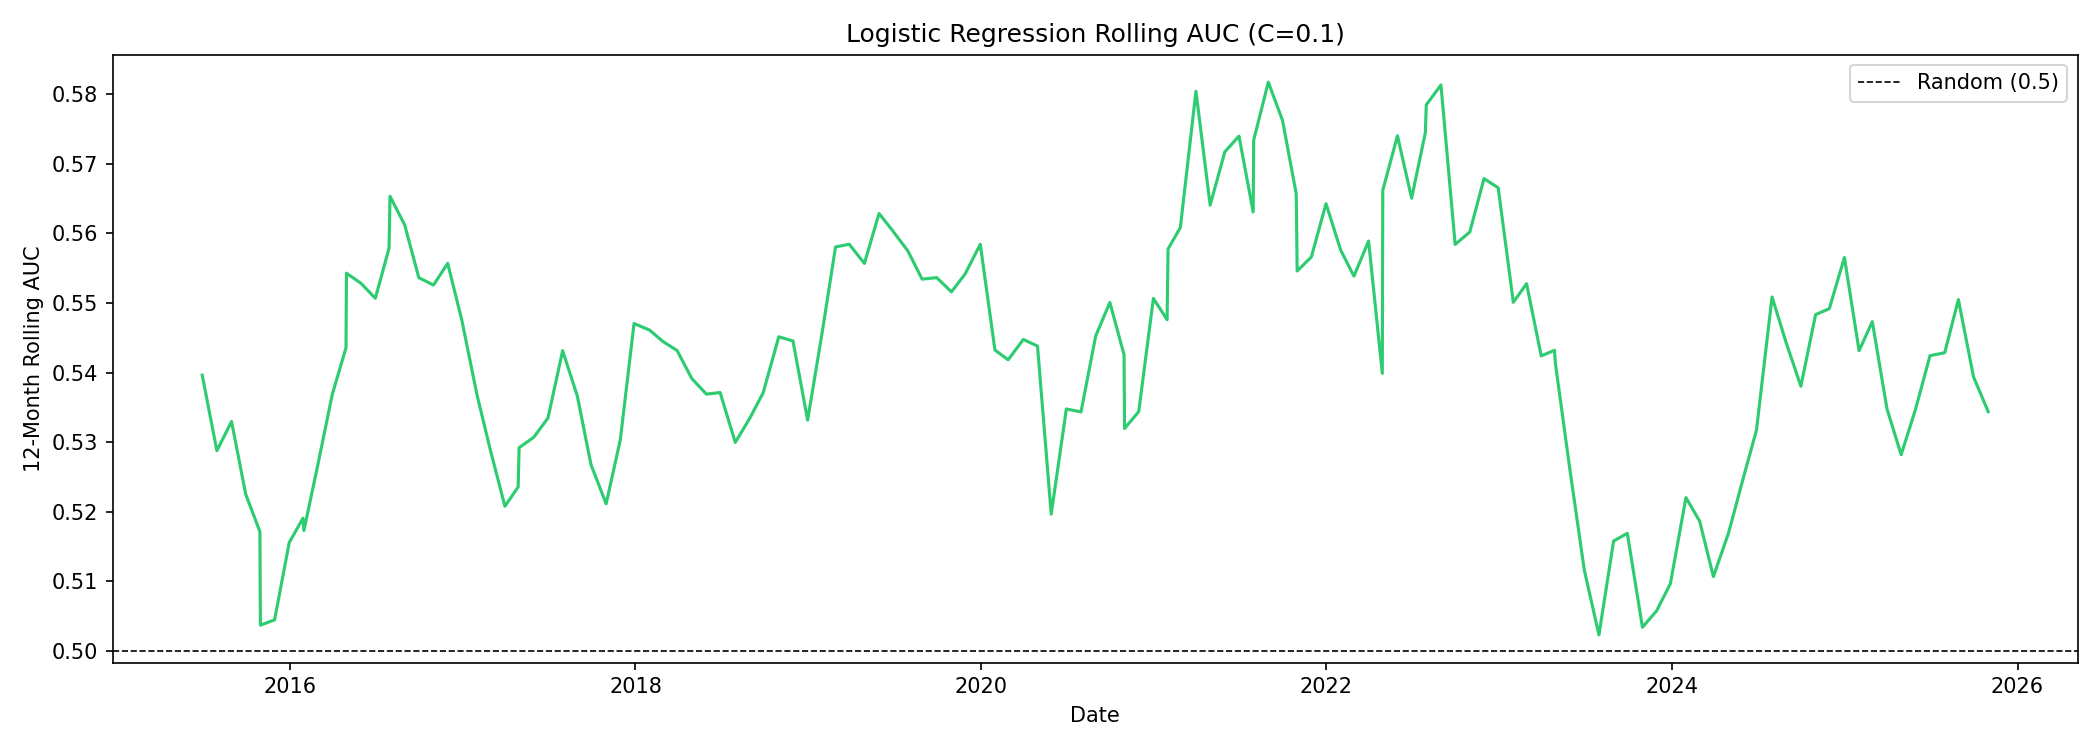
\includegraphics[width=0.8\textwidth]{classification_comparison.png}
    \caption{Rolling 12-month AUC for logistic regression over the evaluation window.}
    \label{fig:rolling_auc}
\end{figure}

% ============================================================
\section{Stochastic Gradient Descent}
\label{sec:sgd}
% ============================================================

Stochastic gradient descent (SGD) provides an alternative optimization strategy that processes training data in small batches rather than computing the full gradient over the entire dataset. This property makes SGD naturally amenable to parallelization and is the workhorse optimizer for large-scale machine learning. We apply mini-batch SGD with L2 regularization to the same return prediction task, focusing on the trade-off between batch size, convergence speed, and predictive accuracy.

\subsection{Methodology}

The SGD regression model minimizes the L2-regularized mean squared error:

\begin{equation}
    \min_{\beta} \frac{1}{|B|} \sum_{i \in B} (y_i - x_i^{\intercal}\beta)^2 + \lambda \|\beta\|_2^2
\end{equation}

where $B$ is a mini-batch of training observations sampled at each iteration. We use scikit-learn's \verb|SGDRegressor| with \verb|partial_fit|, which allows incremental learning over batches. The learning rate is held constant at $\eta = 0.001$, and we evaluate three batch sizes: 64, 256, and 1{,}024.

For convergence analysis, we train each batch-size configuration for 50 epochs on a fixed training set and record the loss at each epoch. For predictive evaluation, we use the same expanding-window framework as the other models, training for 30 epochs at each window step.

\subsection{Results}

Figure~\ref{fig:sgd_convergence} shows the convergence curves for the three batch sizes. Smaller batches (64) converge faster in terms of epochs but require more gradient updates per epoch. All three configurations converge within 30 epochs, justifying our choice of epoch count for the expanding-window evaluation.

\begin{figure}[H]
    \centering
    
\includegraphics[width=0.8\textwidth]{sgd_convergence.png}
    \caption{SGD convergence curves for different batch sizes. Smaller batches converge faster per epoch.}
    \label{fig:sgd_convergence}
\end{figure}

The out-of-sample results are summarized in Table~\ref{tab:sgd_results}. Batch size 64 achieves the highest mean IC (0.0480) and hit rate (66.89\%), while batch size 1{,}024 is $12\times$ faster but sacrifices predictive accuracy (IC = 0.0383). This demonstrates the classic bias-variance trade-off in SGD: smaller batches introduce more stochastic noise per update, which acts as implicit regularization and can improve generalization.

\begin{table}[H]
\centering
\caption{SGD regression results by batch size.}
\label{tab:sgd_results}
\begin{tabular}{lcccc}
\toprule
Batch Size & Mean IC & IC Std & Hit Rate & Time (sec) \\
\midrule
64   & 0.0480 & 0.110 & 66.89\% & 744.5 \\
256  & 0.0459 & 0.111 & 65.54\% & 178.1 \\
1024 & 0.0383 & 0.118 & 64.86\% & 62.0 \\
\bottomrule
\end{tabular}
\end{table}

\begin{figure}[H]
    \centering
    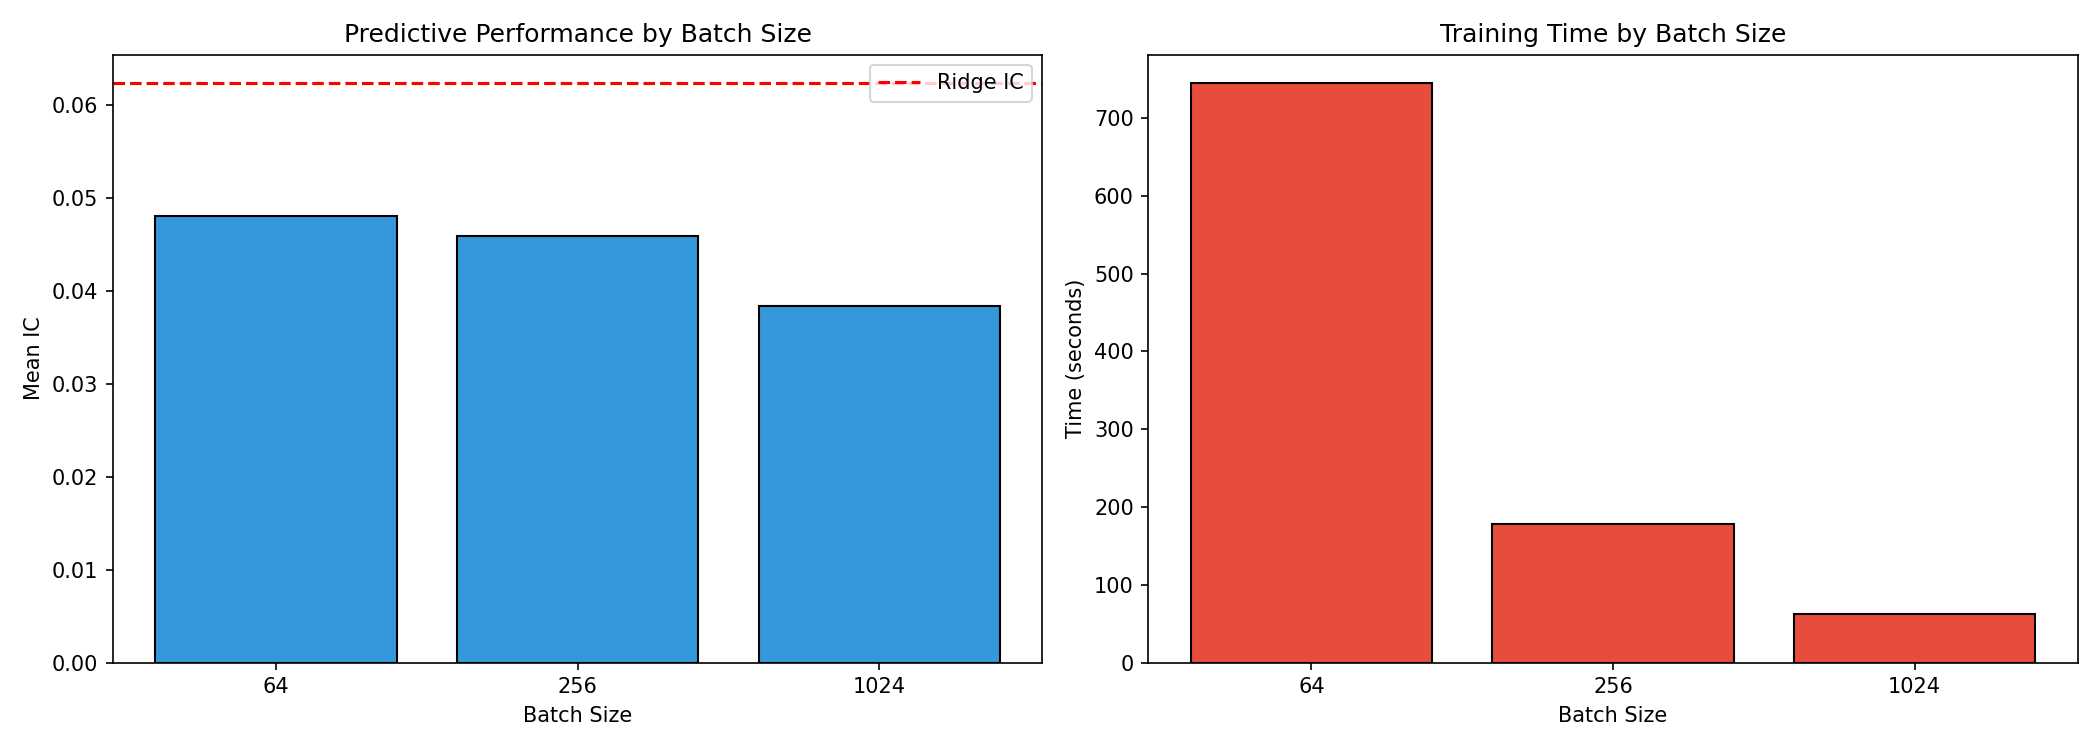
\includegraphics[width=0.8\textwidth]{sgd_batch_comparison.png}
    \caption{Comparison of SGD performance metrics across batch sizes.}
    \label{fig:sgd_batch}
\end{figure}

Even at its best (batch size 64), SGD underperforms both Ridge (IC = 0.0623) and the neural network (IC = 0.0577). This is expected: SGD with a linear model is essentially fitting the same functional form as Ridge but with a noisier optimization procedure. However, SGD's value lies in its scalability---the batch-level computation is trivially parallelizable, and the framework extends naturally to online learning settings where data arrives in streams.

% ============================================================
\section{Neural Networks}
\label{sec:neural_net}
% ============================================================

Neural networks offer the ability to capture nonlinear relationships between features and returns that linear models cannot exploit. We evaluate feedforward neural networks of increasing depth to test whether the cross-sectional return prediction problem contains exploitable nonlinearity, and whether deeper architectures can justify their additional computational cost.

\subsection{Architecture and Training}

We use scikit-learn's \verb|MLPRegressor| with the following configuration: ReLU activation, Adam optimizer, L2 regularization ($\alpha = 0.01$), adaptive learning rate (initial value 0.001), and early stopping with a patience of 10 rounds using a 10\% validation split. Three architectures are evaluated:

\begin{itemize}
    \item \textbf{NN\_32}: One hidden layer with 32 units.
    \item \textbf{NN\_64\_32}: Two hidden layers with 64 and 32 units.
    \item \textbf{NN\_128\_64\_32}: Three hidden layers with 128, 64, and 32 units.
\end{itemize}

All networks are trained using the same expanding-window procedure with a maximum of 200 iterations per window step. The results are reported in Table~\ref{tab:nn_results}, with Ridge included as a linear baseline.

\begin{table}[H]
\centering
\caption{Neural network architecture comparison. Ridge is included as a linear baseline.}
\label{tab:nn_results}
\begin{tabular}{lcccc}
\toprule
Model & Mean IC & IC Std & Hit Rate & Time (sec) \\
\midrule
Ridge (baseline)  & 0.0623 & 0.119 & 72.97\% & 2.1 \\
NN\_32            & 0.0480 & 0.092 & 71.62\% & 270.1 \\
NN\_64\_32        & 0.0577 & 0.102 & 73.65\% & 309.4 \\
NN\_128\_64\_32   & 0.0593 & 0.101 & 72.30\% & 3{,}710.1 \\
\bottomrule
\end{tabular}
\end{table}

\subsection{Architecture Selection and Nonlinearity}

We select NN\_64\_32 as the primary neural network model. Although NN\_128\_64\_32 achieves a marginally higher IC (0.0593 vs.\ 0.0577), NN\_64\_32 achieves the highest hit rate (73.65\%) and is $12\times$ faster. The diminishing returns from additional depth suggest that the exploitable nonlinearity in this dataset is moderate.

To further investigate the nonlinearity hypothesis, we split the evaluation window into an early period (2015--2019) and a late period (2020--2025) and compare how each model's IC changes over time. All models improve in the late period, but the neural networks show larger gains ($+0.018$ to $+0.021$) compared to Ridge ($+0.015$). This modest differential suggests that nonlinear patterns in the cross-section have become slightly more pronounced in recent years, consistent with findings in the broader literature on machine learning in finance \cite{gu2020}.

\begin{figure}[H]
    \centering
    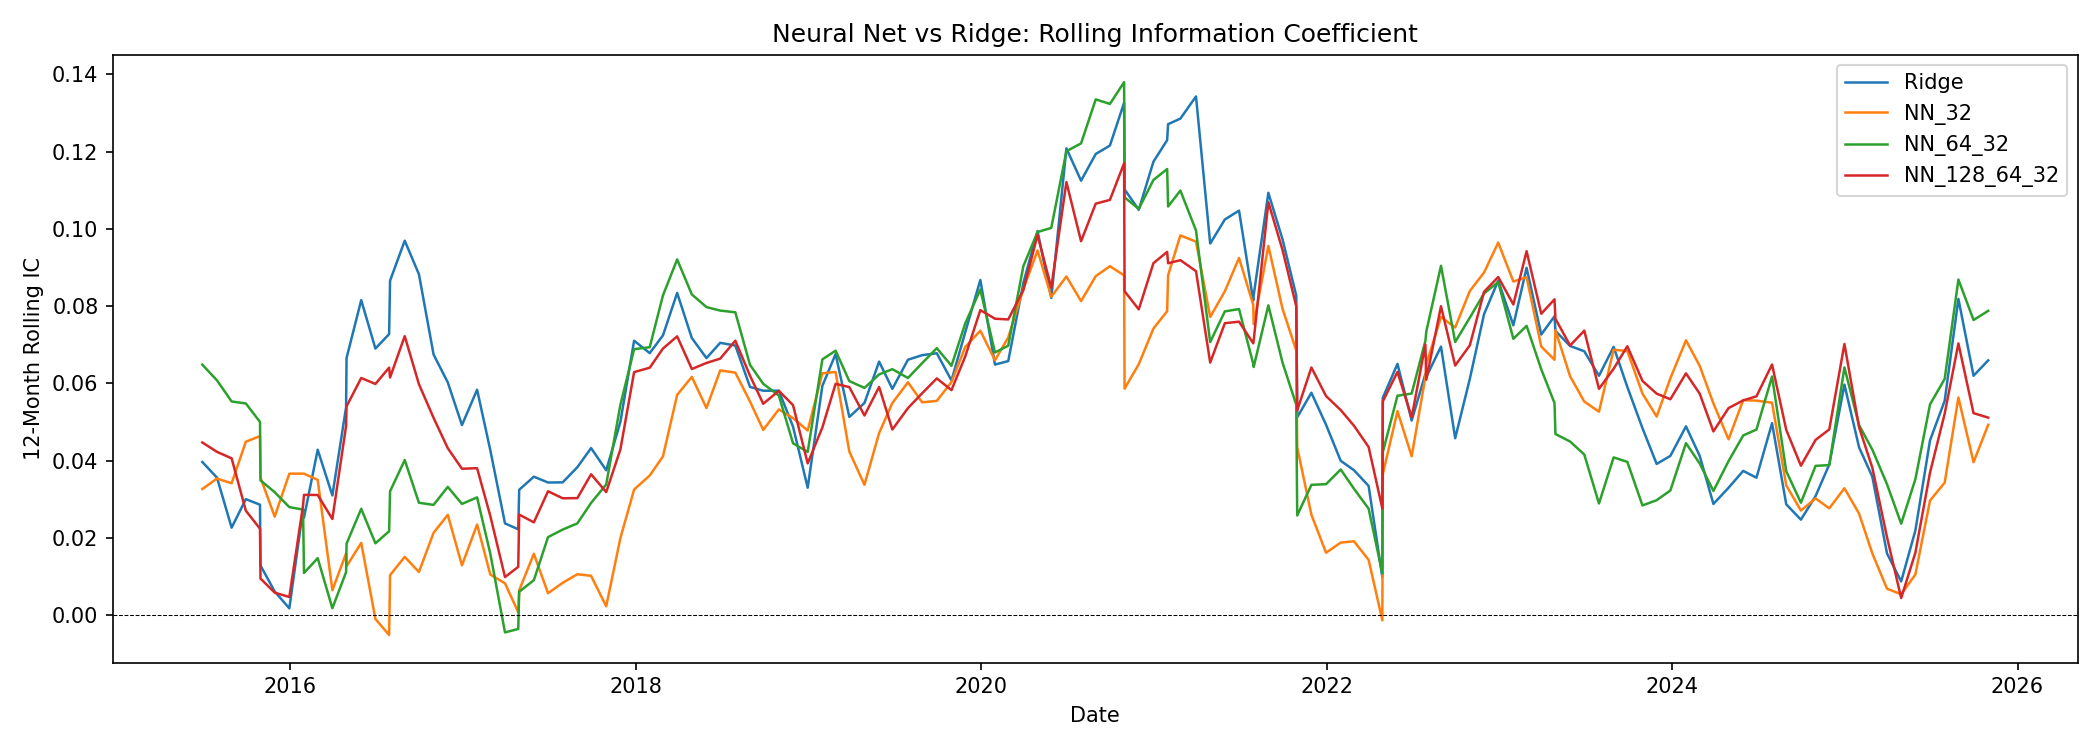
\includegraphics[width=0.8\textwidth]{nn_rolling_ic.png}
    \caption{Rolling IC for neural network architectures compared to the Ridge baseline.}
    \label{fig:nn_rolling_ic}
\end{figure}

\begin{figure}[H]
    \centering
    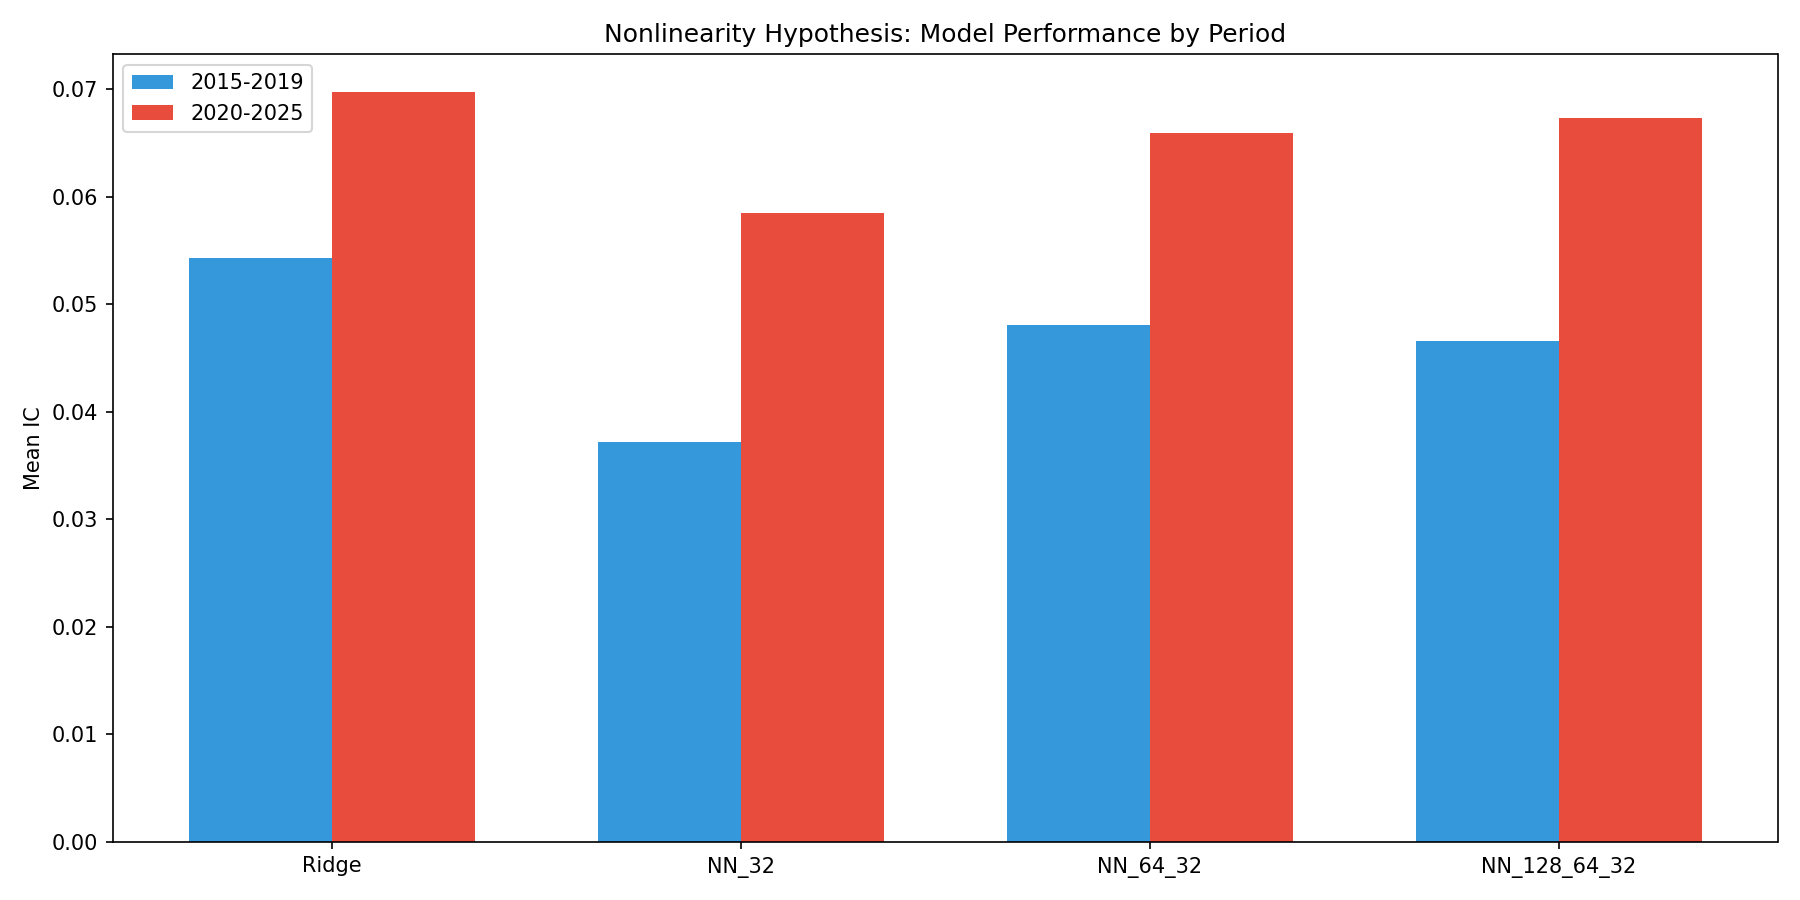
\includegraphics[width=0.7\textwidth]{nn_vs_linear_by_period.png}
    \caption{Mean IC in the early (2015--2019) and late (2020--2025) evaluation periods. All models improve over time, with neural networks showing slightly larger gains.}
    \label{fig:nn_vs_linear}
\end{figure}

\subsection{Parallelism}

The neural network benefits most from parallelization among all models tested. At 16 cores, the Spark-distributed NN\_64\_32 pipeline achieves a $4.37\times$ speedup (reducing wall-clock time from 814.6 seconds to 186.6 seconds), compared to $2.29\times$ for Lasso, $1.28\times$ for Ridge, and $1.10\times$ for Fama--MacBeth (Figure~\ref{fig:speedup}). This is because NN training involves iterative backpropagation for up to 200 iterations per window, making each task compute-intensive enough that the parallelization overhead is amortized. The near-linear scaling between 1 and 4 cores, with diminishing returns above 8 cores, is consistent with Amdahl's law applied to the sequential overhead of Spark task scheduling and result aggregation.

% ============================================================
\section{Portfolio Construction and Backtest}
\label{sec:portfolio}
% ============================================================

To translate predictive signals into economic value, we construct long-short decile portfolios for each of the four primary models (Fama--MacBeth, Ridge, Lasso, NN\_64\_32). At each test month, stocks are sorted by predicted return, and the portfolio goes long the top decile (approximately 50 stocks) and short the bottom decile. Portfolio returns are computed as the equal-weighted mean return of the long leg minus the equal-weighted mean return of the short leg. No leverage, margin, or borrowing costs are assumed in the baseline analysis; transaction costs are addressed separately in Section~\ref{sec:turnover}.

\begin{table}[H]
\centering
\caption{Long-short decile portfolio performance over 148 out-of-sample months. An equal-weighted S\&P 500 benchmark is included for reference.}
\label{tab:portfolio}
\begin{tabular}{lccccc}
\toprule
Model & Ann.\ Return & Ann.\ Vol & Sharpe & Max DD & Win Rate \\
\midrule
Fama--MacBeth & 28.73\% & 14.15\% & 2.03 & $-11.52\%$ & 77.03\% \\
Ridge         & 30.90\% & 14.86\% & 2.08 & $-10.73\%$ & 75.68\% \\
Lasso         & 28.92\% & 15.29\% & 1.89 & $-18.37\%$ & 72.30\% \\
NN\_64\_32    & 28.03\% & 12.33\% & \textbf{2.27} & $\mathbf{-5.76\%}$ & \textbf{77.70\%} \\
\midrule
Equal Weight  & 14.44\% & 9.97\%  & 1.45 & $-14.61\%$ & 74.32\% \\
\bottomrule
\end{tabular}
\end{table}

All four models approximately double the Sharpe ratio of the equal-weight benchmark. Ridge achieves the highest annualized return (30.90\%), but the neural network delivers the best risk-adjusted performance: the highest Sharpe ratio (2.27), the lowest maximum drawdown ($-5.76\%$), the lowest volatility (12.33\%), and the highest win rate (77.70\%). The neural network's superior risk management is a recurring theme throughout our analysis.

\begin{figure}[H]
    \centering
    
\includegraphics[width=0.85\textwidth]{cumulative_returns.png}
    \caption{Cumulative returns of long-short decile portfolios for all four models over the 148-month evaluation period.}
    \label{fig:cumulative_returns}
\end{figure}

\begin{figure}[H]
    \centering
    
\includegraphics[width=0.85\textwidth]{drawdown.png}
    \caption{Drawdown profiles for each model's long-short portfolio.}
    \label{fig:drawdown}
\end{figure}

% ============================================================
\section{Model Comparison and Analysis}
\label{sec:comparison}
% ============================================================

This section presents a comprehensive comparison of the four primary models across seven dimensions: statistical significance, quintile spread analysis, market regime resilience, signal decay, portfolio turnover and transaction costs, feature importance, and Fama--French factor attribution.

% ------------------------------------------------------------
\subsection{Statistical Significance}
\label{sec:significance}
% ------------------------------------------------------------

Table~\ref{tab:ic_ir} reports the IC-based Information Ratio (IC\_IR = Mean IC / IC Std) and the $t$-statistic for each model's mean IC being different from zero. All four models achieve highly significant positive ICs ($t > 4.8$, $p < 0.001$). The neural network achieves the highest IC\_IR (0.565) and $t$-statistic (6.88), indicating that it is the most consistent predictor per unit of IC volatility despite having a lower raw IC than Ridge.

\begin{table}[H]
\centering
\caption{Information Coefficient summary and Information Ratio for each model.}
\label{tab:ic_ir}
\begin{tabular}{lccccc}
\toprule
Model & Mean IC & IC Std & IC\_IR & $t$-stat & Hit Rate \\
\midrule
Fama--MacBeth & 0.0602 & 0.111 & 0.544 & 6.61 & 70.95\% \\
Ridge         & 0.0623 & 0.119 & 0.525 & 6.39 & 72.97\% \\
Lasso         & 0.0512 & 0.129 & 0.396 & 4.82 & 64.19\% \\
NN\_64\_32    & 0.0577 & 0.102 & \textbf{0.565} & \textbf{6.88} & \textbf{73.65\%} \\
\bottomrule
\end{tabular}
\end{table}

To determine whether the differences between models are statistically significant, we conduct pairwise paired $t$-tests on monthly ICs and Diebold--Mariano (DM) tests \cite{diebold1995} on squared prediction errors. The results are summarized in Table~\ref{tab:significance}.

\begin{table}[H]
\centering
\caption{Pairwise model comparison: paired $t$-test on monthly ICs and Diebold--Mariano test on squared prediction errors. Significant results ($p < 0.05$) are bolded.}
\label{tab:significance}
\begin{tabular}{llcccc}
\toprule
Model A & Model B & IC $t$-stat & IC $p$-val & DM stat & DM $p$-val \\
\midrule
FM    & Ridge   & $-0.94$ & 0.351 & \textbf{2.16} & \textbf{0.031} \\
FM    & Lasso   & \textbf{2.41} & \textbf{0.017} & \textbf{2.04} & \textbf{0.041} \\
FM    & NN      & 0.49 & 0.622 & 1.70 & 0.089 \\
Ridge & Lasso   & \textbf{3.65} & \textbf{$<$0.001} & \textbf{$-2.27$} & \textbf{0.024} \\
Ridge & NN      & 0.94 & 0.349 & \textbf{$-2.88$} & \textbf{0.004} \\
Lasso & NN      & $-1.04$ & 0.299 & \textbf{$-2.13$} & \textbf{0.034} \\
\bottomrule
\end{tabular}
\end{table}

Ridge significantly outperforms Lasso by both tests ($p < 0.001$ by IC $t$-test, $p = 0.024$ by DM). Ridge also outperforms Fama--MacBeth by the DM test ($p = 0.031$) but not by the IC $t$-test ($p = 0.351$). The comparison between Ridge and NN is nuanced: Ridge is a significantly better point predictor by the DM test ($p = 0.004$), but the IC difference is not significant ($p = 0.349$), and the NN delivers superior portfolio-level performance (higher Sharpe, lower drawdown). This suggests that the NN's advantage lies not in raw predictive accuracy but in the nature of its errors---it may make smaller errors on the stocks that matter most for portfolio construction.

\begin{figure}[H]
    \centering
    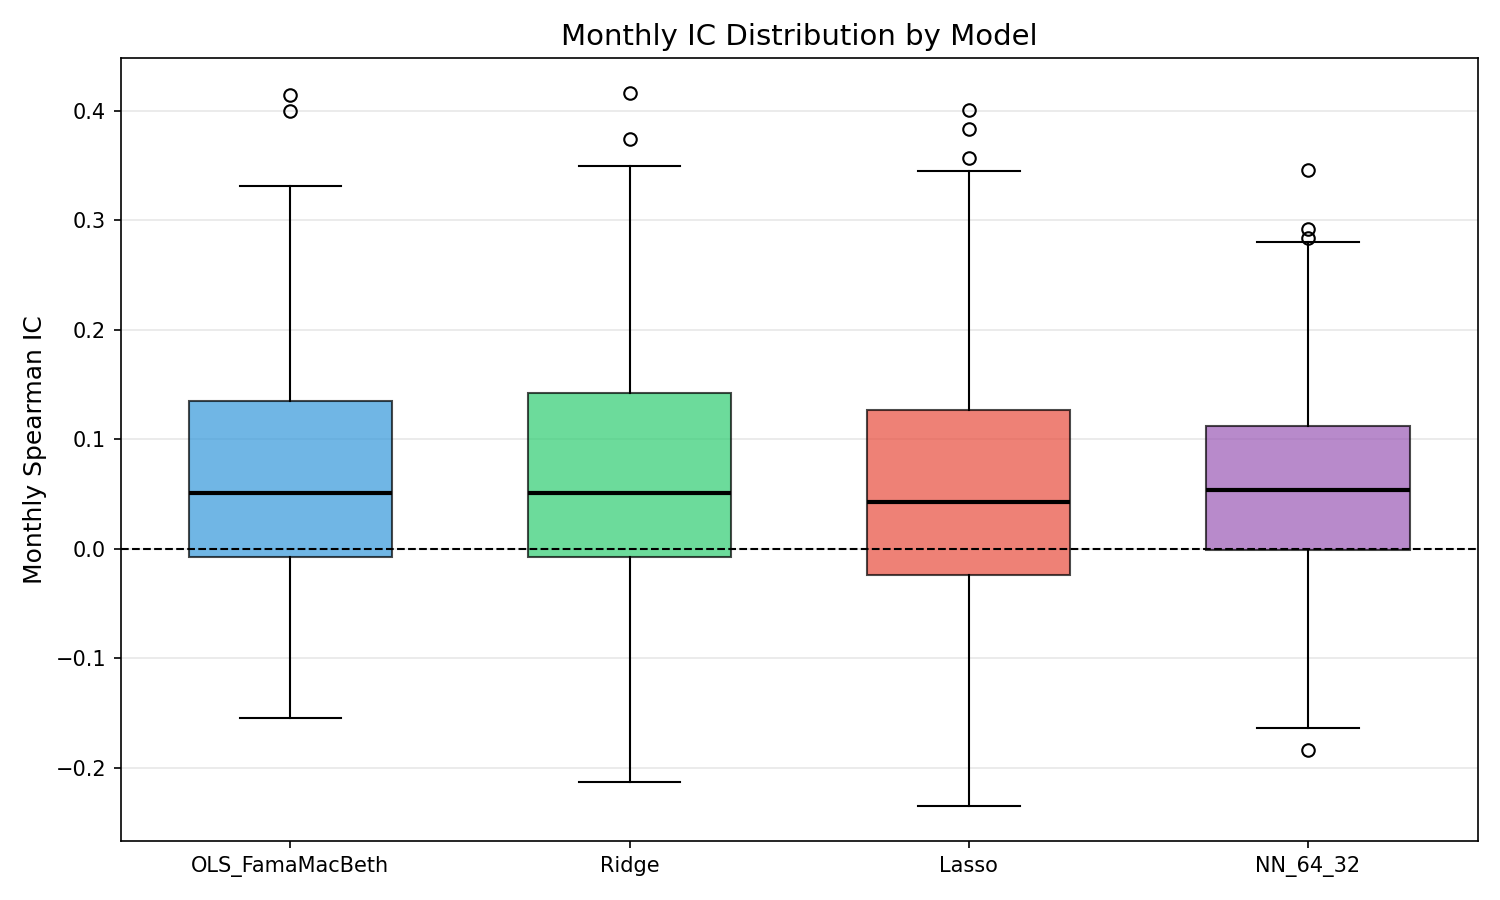
\includegraphics[width=0.8\textwidth]{ic_boxplot.png}
    \caption{Distribution of monthly Information Coefficients across models.}
    \label{fig:ic_boxplot}
\end{figure}

\begin{figure}[H]
    \centering
    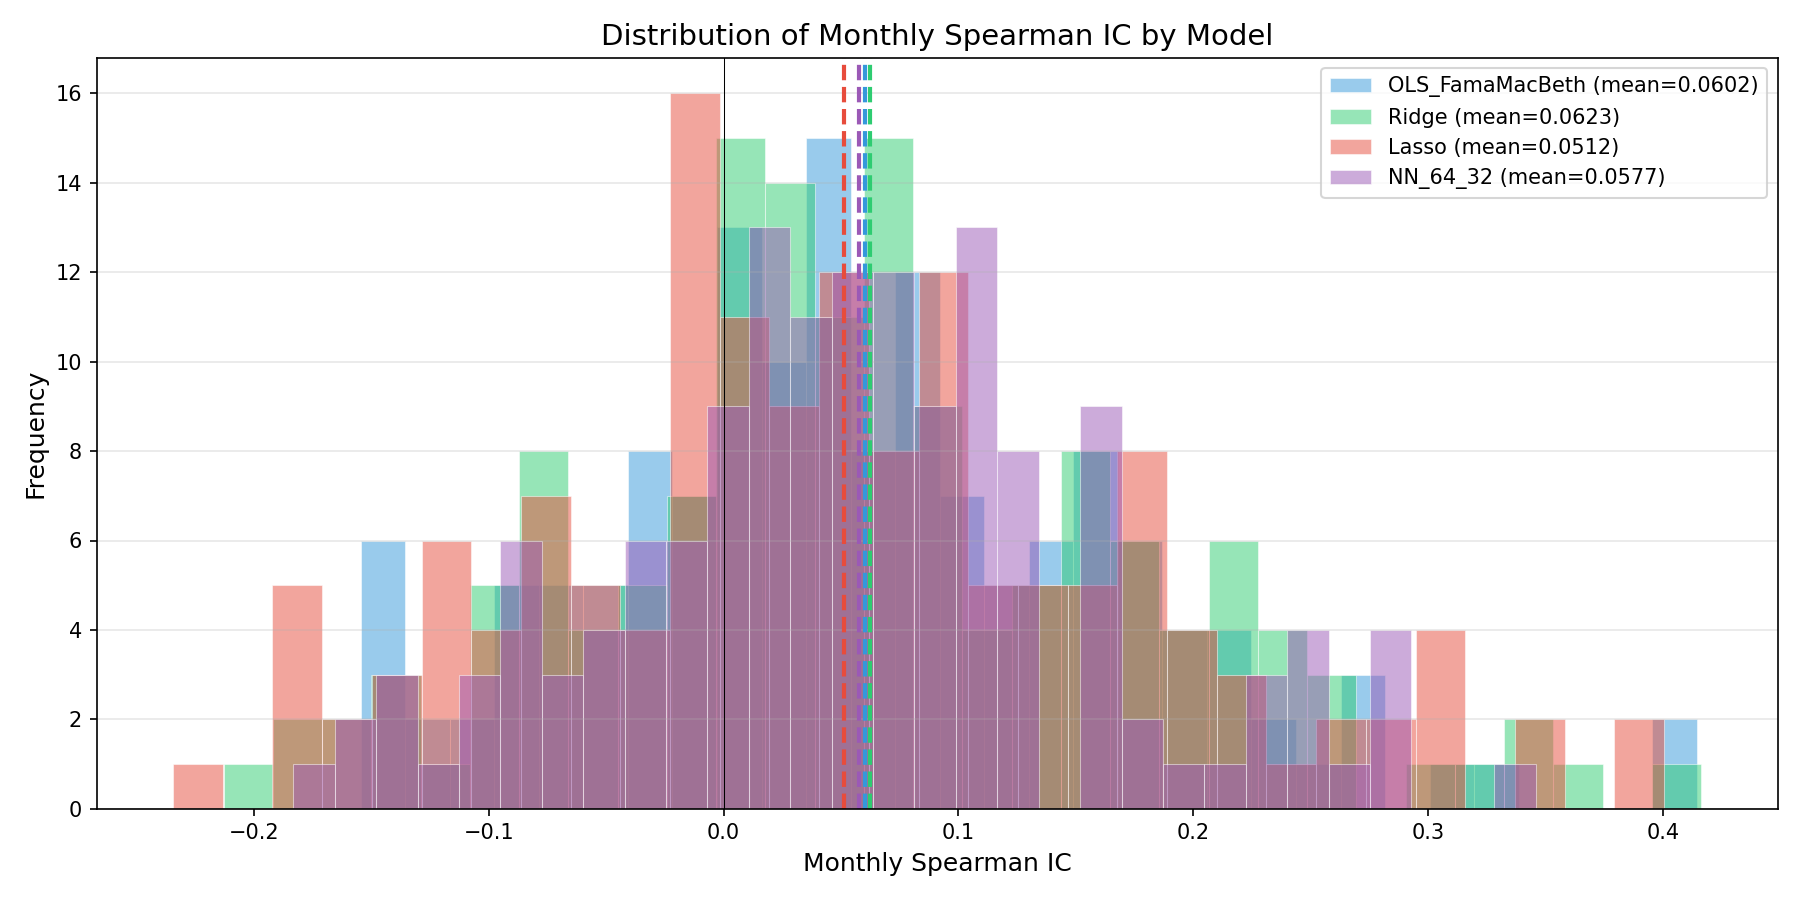
\includegraphics[width=0.8\textwidth]{ic_histogram.png}
    \caption{Overlaid histograms of monthly IC distributions for all four models.}
    \label{fig:ic_histogram}
\end{figure}

% ------------------------------------------------------------
\subsection{Quintile Spread Analysis}
\label{sec:quintile}
% ------------------------------------------------------------

A strong predictive model should produce monotonically decreasing realized returns from the top to the bottom predicted-return quintile. Table~\ref{tab:quintile} reports the mean monthly return for each quintile, the Q1$-$Q5 spread, and its $t$-statistic.

\begin{table}[H]
\centering
\caption{Mean monthly quintile returns (\%). All models exhibit perfect monotonicity.}
\label{tab:quintile}
\begin{tabular}{lcccccccc}
\toprule
Model & Q1 (Top) & Q2 & Q3 & Q4 & Q5 (Bot) & Spread & $t$-stat & Mono. \\
\midrule
FM    & 2.40 & 1.31 & 1.01 & 0.71 & 0.60 & 1.80 & 7.26 & \checkmark \\
Ridge & 2.41 & 1.33 & 0.99 & 0.76 & 0.55 & 1.86 & 7.26 & \checkmark \\
Lasso & 2.37 & 1.26 & 0.99 & 0.77 & 0.65 & 1.72 & 6.33 & \checkmark \\
NN    & 2.36 & 1.21 & 0.96 & 0.94 & 0.57 & 1.80 & \textbf{8.16} & \checkmark \\
\bottomrule
\end{tabular}
\end{table}

All four models produce perfectly monotonic quintile returns with highly significant spreads ($t > 6.3$). The neural network achieves the highest spread $t$-statistic (8.16), indicating that its Q1$-$Q5 spread is the most consistent across time despite having a slightly narrower raw spread than Ridge. This is consistent with the NN's lower IC standard deviation and higher IC\_IR.

\begin{figure}[H]
    \centering
    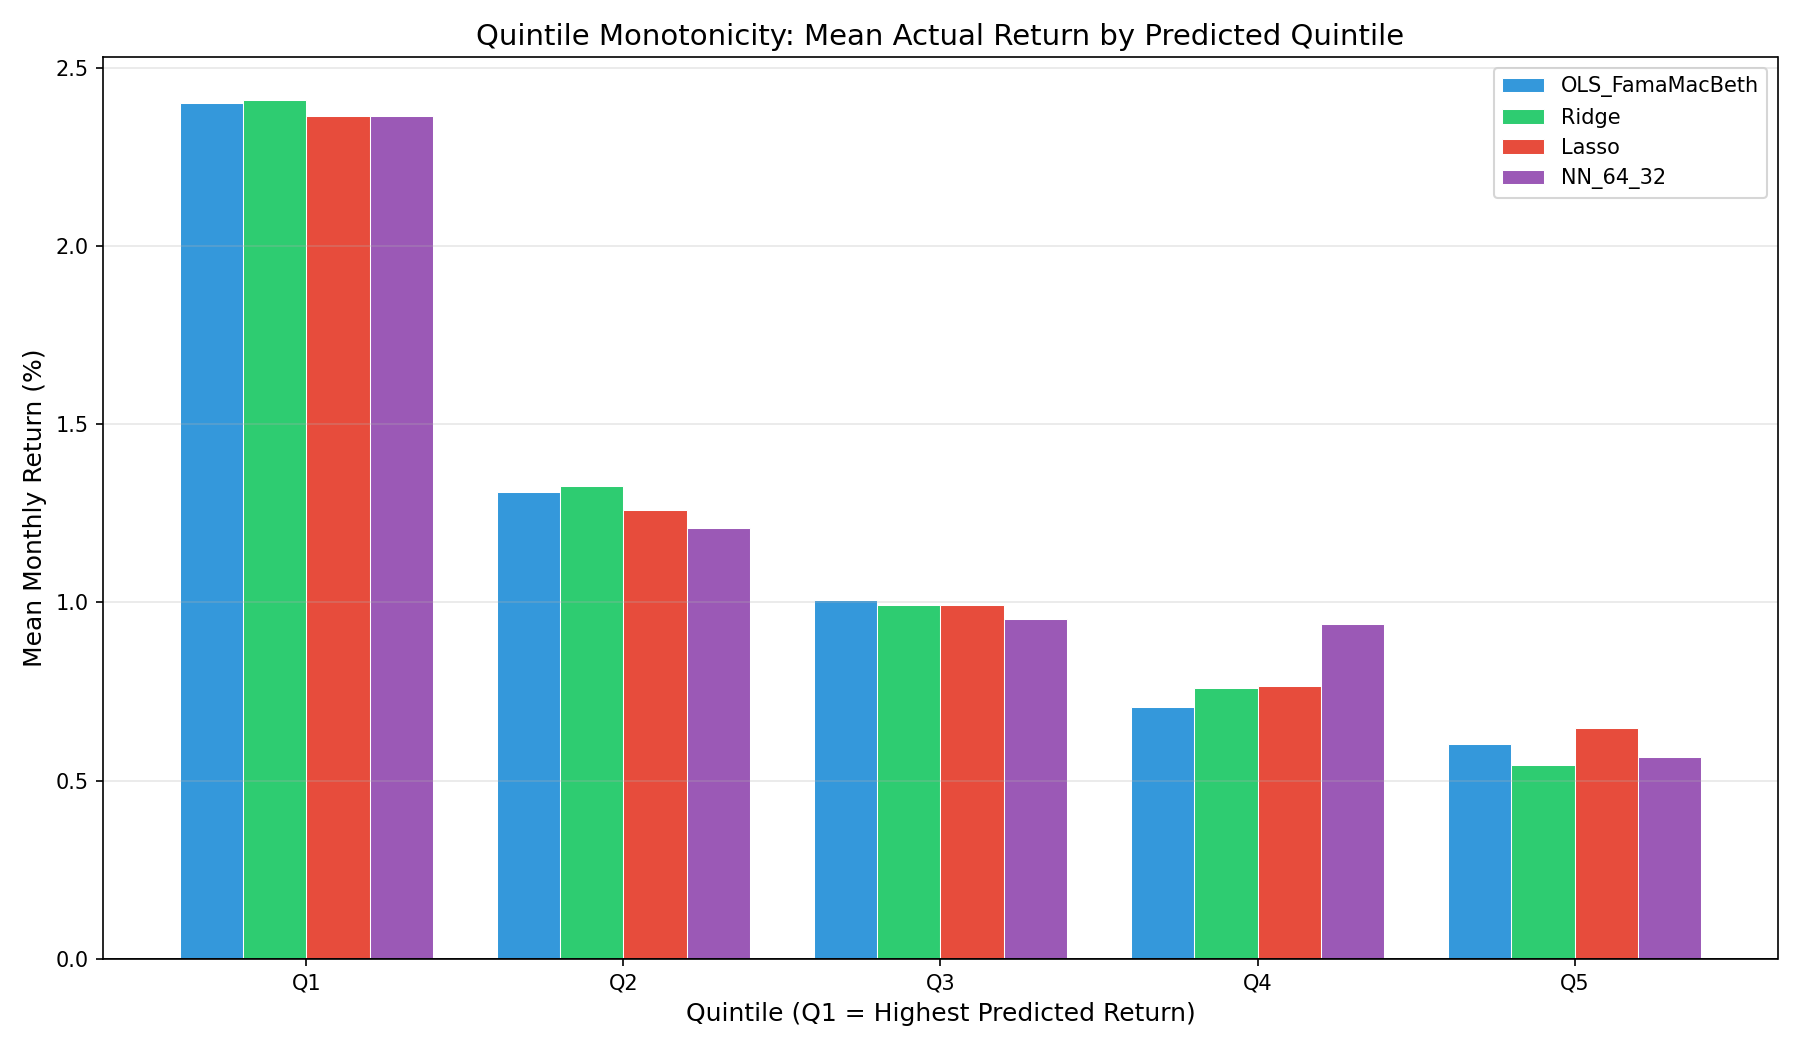
\includegraphics[width=0.75\textwidth]{quintile_monotonicity.png}
    \caption{Mean monthly returns by predicted-return quintile for each model.}
    \label{fig:quintile}
\end{figure}

% ------------------------------------------------------------
\subsection{Market Regime Analysis}
\label{sec:regime}
% ------------------------------------------------------------

We segment the evaluation period into three market regimes based on trailing 12-month S\&P 500 returns: Bull (top quartile, 36 months), Neutral (middle 50\%, 109 months), and Crash (bottom quartile, 3 months). Table~\ref{tab:regime} reports the annualized return and Sharpe ratio for each model under each regime.

\begin{table}[H]
\centering
\caption{Portfolio performance by market regime. The Crash period comprises 3 months (including March 2020).}
\label{tab:regime}
\begin{tabular}{llrrrr}
\toprule
Regime & Metric & FM & Ridge & Lasso & NN \\
\midrule
\multirow{2}{*}{Bull}    & Ann.\ Return & 34.63\% & 33.71\% & 34.87\% & 30.04\% \\
                          & Sharpe       & 2.57    & 2.61    & 2.52    & \textbf{2.80} \\
\midrule
\multirow{2}{*}{Neutral} & Ann.\ Return & 28.48\% & 31.74\% & 27.59\% & 26.88\% \\
                          & Sharpe       & 2.00    & 2.07    & 1.76    & \textbf{2.13} \\
\midrule
\multirow{2}{*}{Crash}   & Ann.\ Return & $-32.98\%$ & $-33.42\%$ & $+5.77\%$ & $\mathbf{+45.37\%}$ \\
                          & Sharpe       & $-3.10$ & $-4.20$ & 0.28 & $\mathbf{+1.99}$ \\
\bottomrule
\end{tabular}
\end{table}

The most striking result is the neural network's crash resilience. During the three crash months, the NN portfolio generated a $+45.37\%$ annualized return (Sharpe 1.99), while the linear models (FM and Ridge) suffered severe losses exceeding $-30\%$ annualized. Lasso also survived the crash (return $+5.77\%$), likely because its sparse feature set avoided factors that reversed during the downturn. The NN's ability to maintain positive returns during extreme market stress is a major practical advantage and likely explains its superior maximum drawdown ($-5.76\%$ vs.\ $-10.73\%$ for Ridge).

\begin{figure}[H]
    \centering
    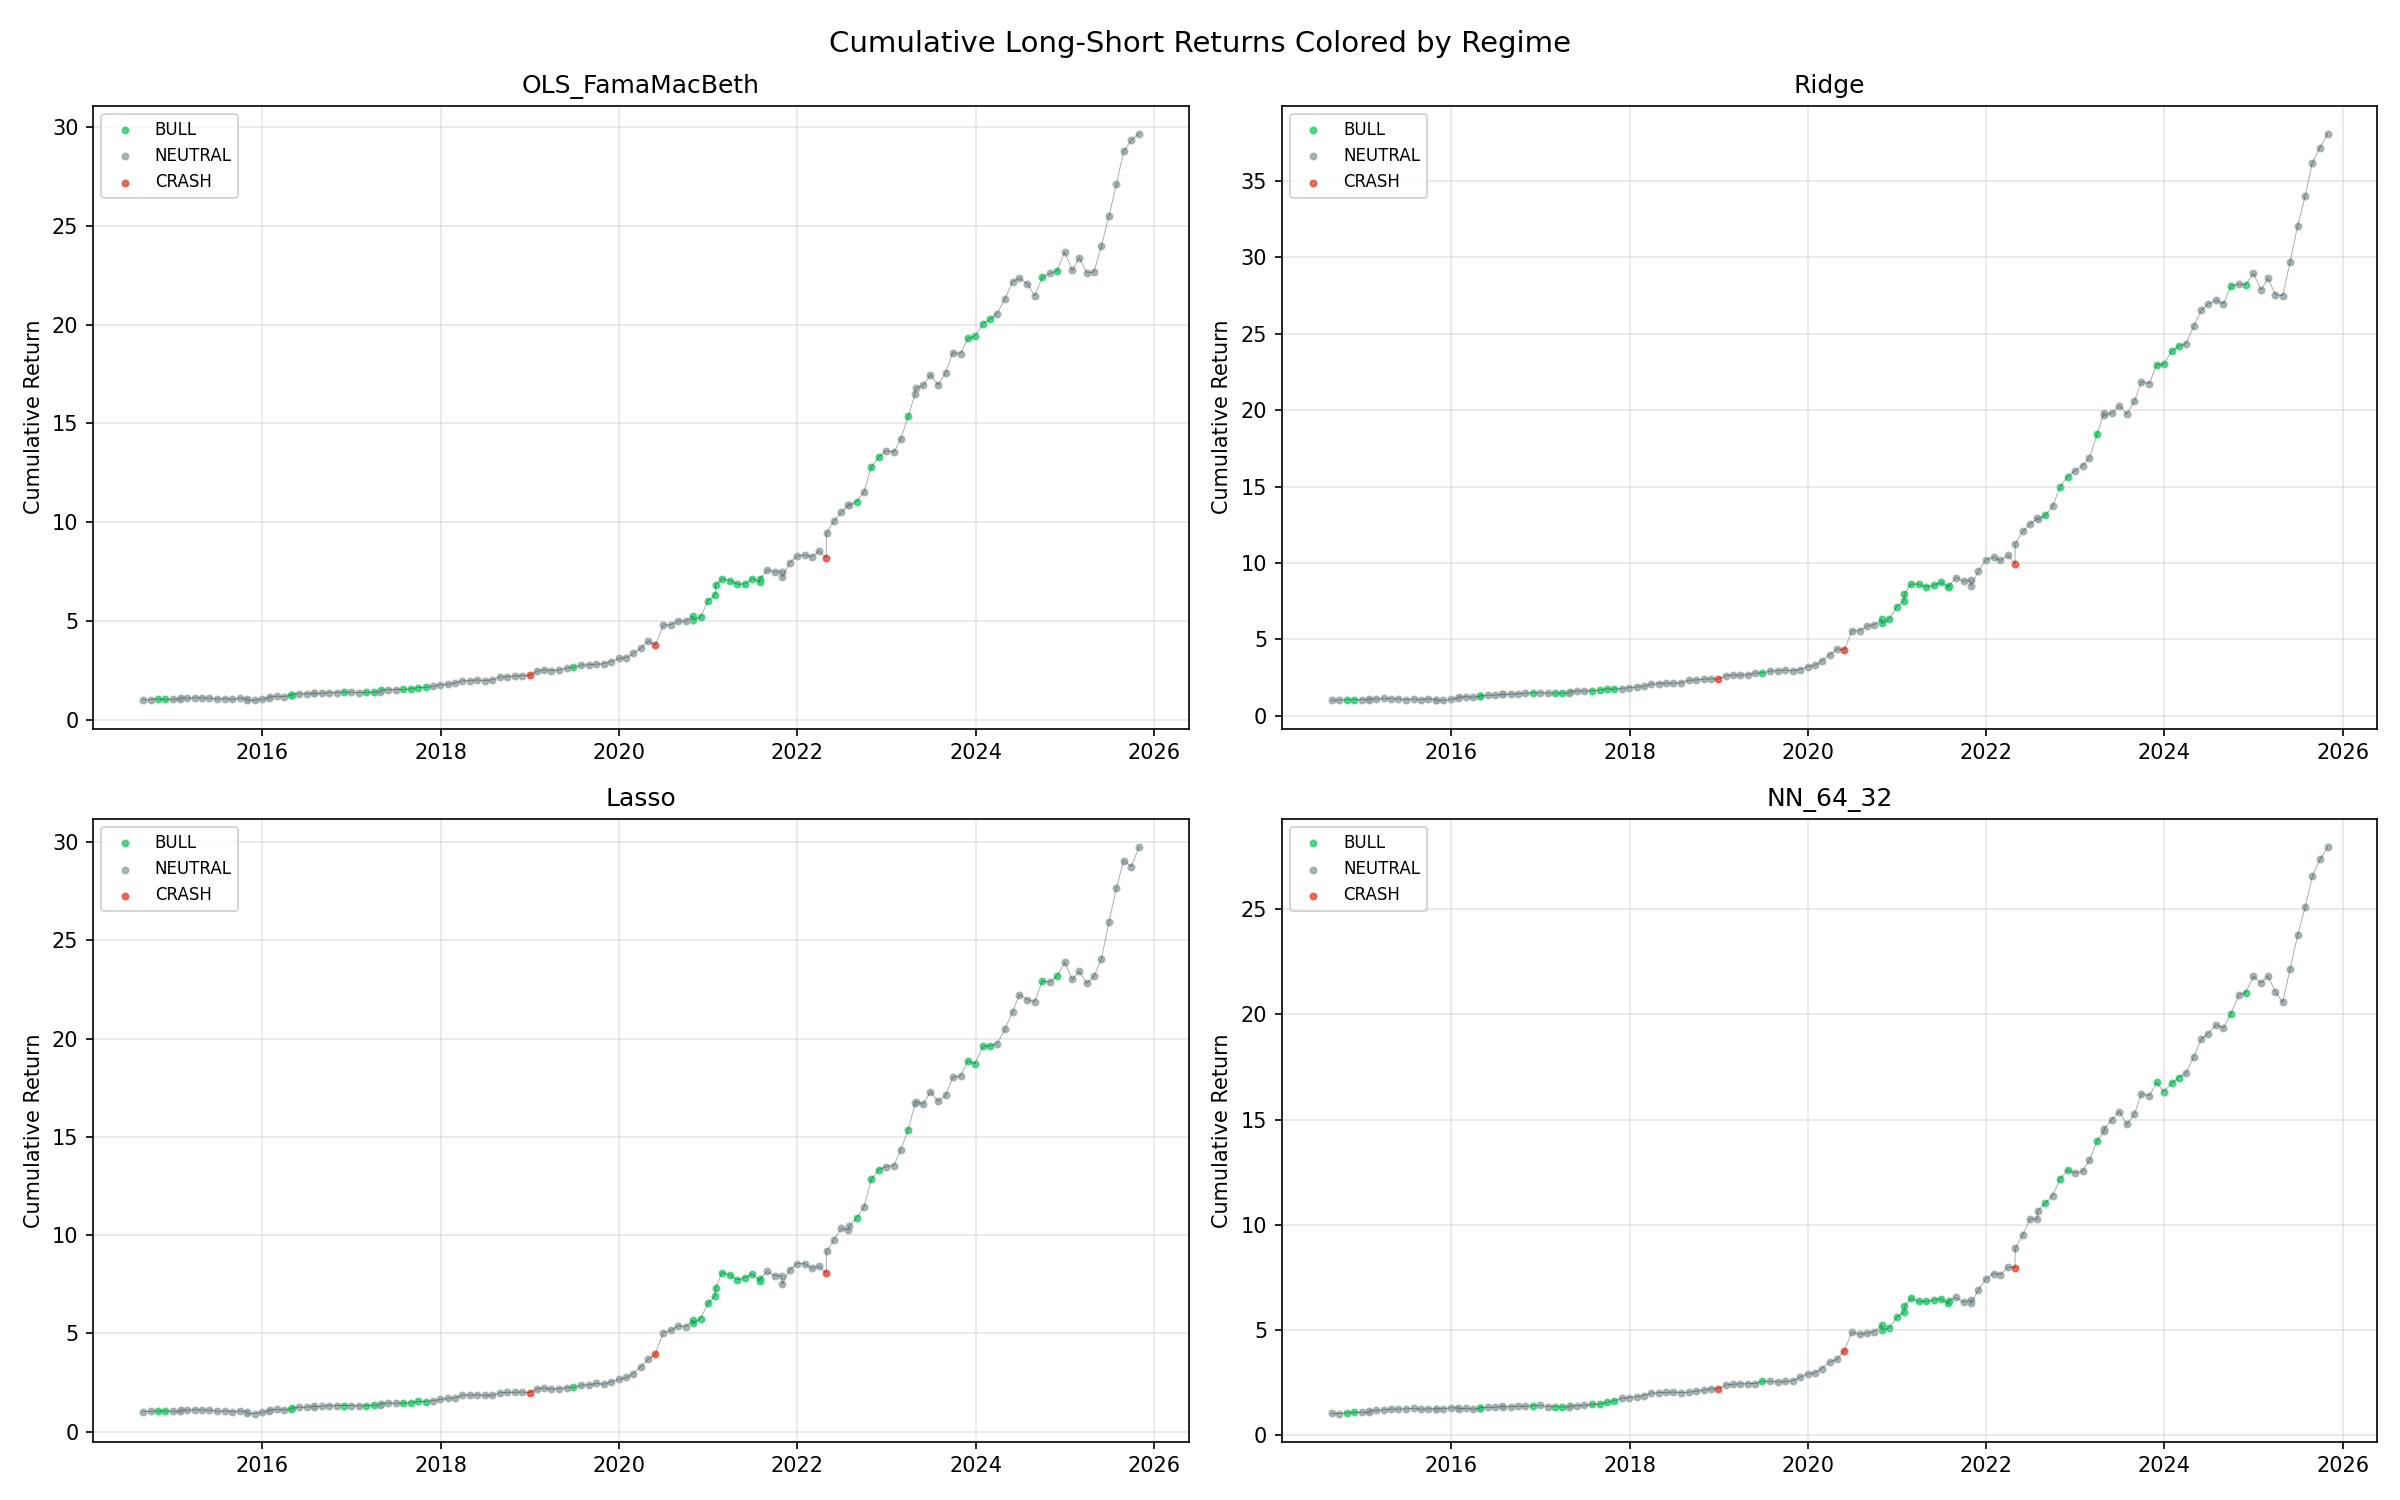
\includegraphics[width=0.85\textwidth]{cumulative_by_regime.png}
    \caption{Cumulative portfolio returns segmented by market regime.}
    \label{fig:cumulative_regime}
\end{figure}

\begin{figure}[H]
    \centering
    \begin{minipage}[t]{0.48\textwidth}
        \centering
        
\includegraphics[width=\textwidth]{sharpe_by_regime.png}
        \caption{Sharpe ratio by regime.}
        \label{fig:sharpe_regime}
    \end{minipage}
    \hfill
    \begin{minipage}[t]{0.48\textwidth}
        \centering
        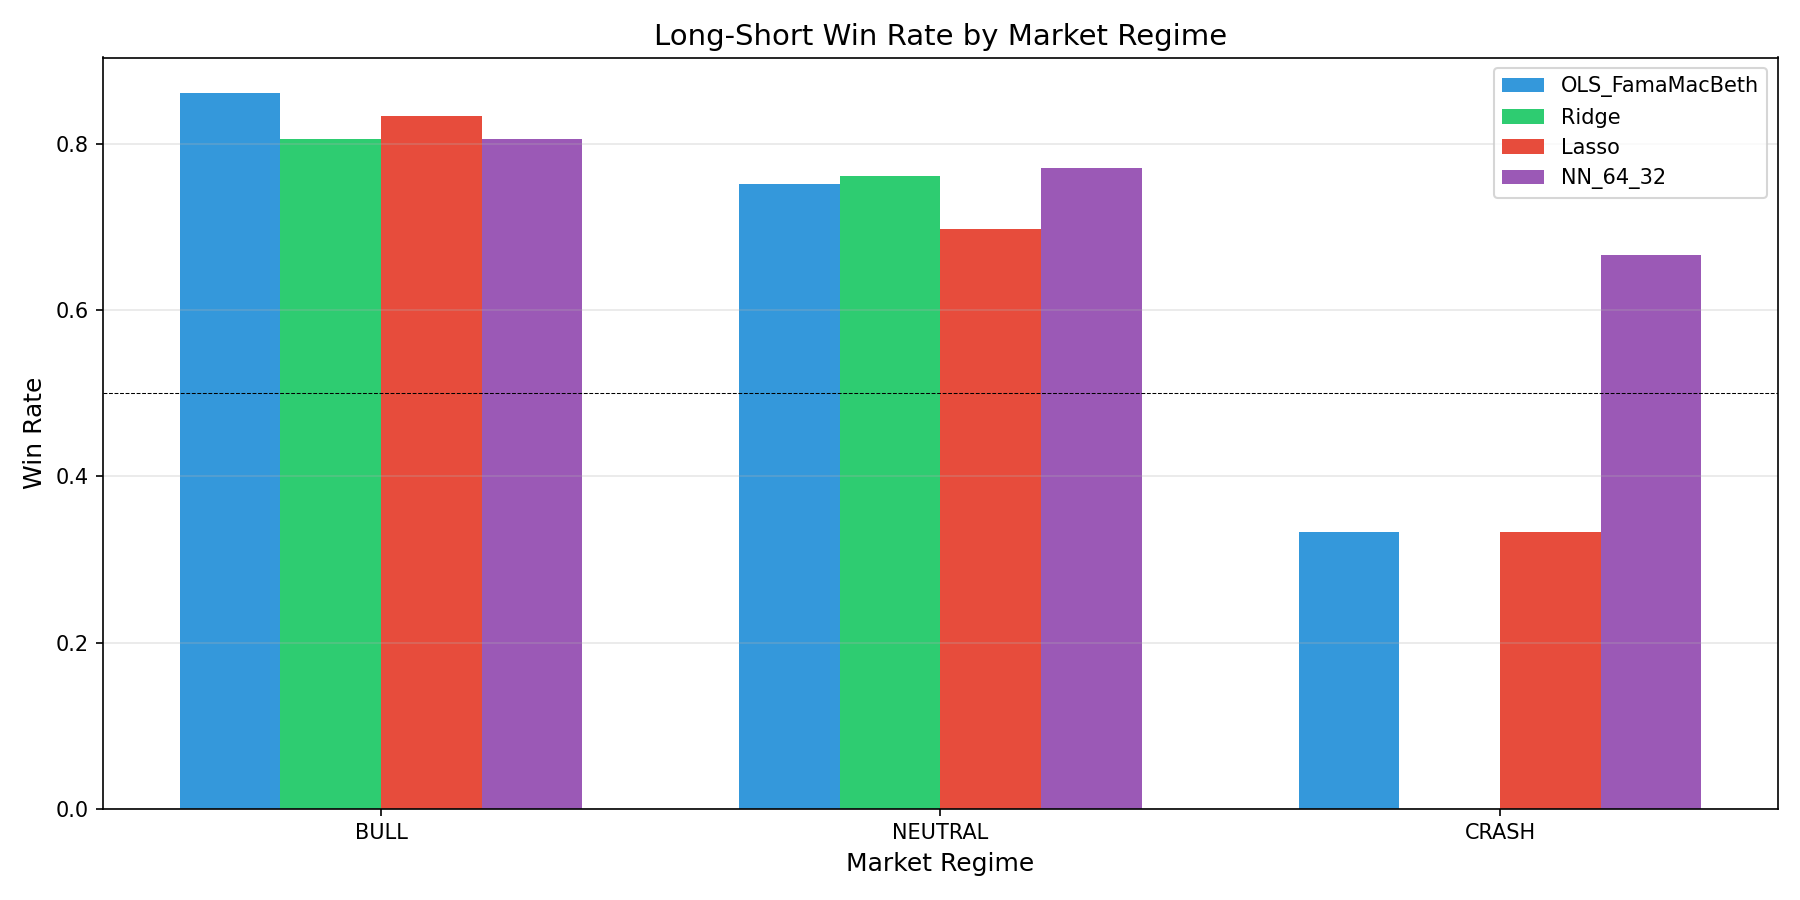
\includegraphics[width=\textwidth]{winrate_by_regime.png}
        \caption{Win rate by regime.}
        \label{fig:winrate_regime}
    \end{minipage}
\end{figure}

% ------------------------------------------------------------
\subsection{Signal Decay}
\label{sec:decay}
% ------------------------------------------------------------

We examine how the predictive power of each model's signal decays as the holding period increases from 1 to 12 months. For each model, we compute the Spearman IC between predictions made at time $t$ and realized returns at horizons $t+1, t+2, \ldots, t+12$.

Counterintuitively, the IC \textit{increases} with holding period for all models (Figure~\ref{fig:decay}), reaching a peak at the 12-month horizon. For Ridge, the IC rises from 0.062 at 1 month to 0.140 at 12 months. This suggests that the features we use---predominantly fundamental and valuation ratios---capture slow-moving value characteristics that are more predictive of cumulative long-run returns than of noisy month-to-month price changes. The neural network shows a similar but less pronounced pattern (0.058 to 0.109), suggesting that some of its signal is more short-lived, possibly due to its reliance on momentum and volatility features.

\begin{figure}[H]
    \centering
    
\includegraphics[width=0.8\textwidth]{factor_decay_curves.png}
    \caption{Information Coefficient by holding period (months). Signals strengthen with longer horizons, consistent with value-oriented factor sets.}
    \label{fig:decay}
\end{figure}

% ------------------------------------------------------------
\subsection{Turnover and Transaction Costs}
\label{sec:turnover}
% ------------------------------------------------------------

Portfolio turnover is the fraction of stocks in the long or short leg that change from one month to the next. High turnover increases transaction costs and can erode returns in practice. Table~\ref{tab:turnover} reports the average monthly turnover for each model.

\begin{table}[H]
\centering
\caption{Average monthly portfolio turnover (\%) over 147 rebalancing months.}
\label{tab:turnover}
\begin{tabular}{lccc}
\toprule
Model & Long Turnover & Short Turnover & Total Turnover \\
\midrule
Fama--MacBeth & 23.79\% & 22.12\% & 22.96\% \\
Ridge         & 22.63\% & 22.10\% & 22.36\% \\
Lasso         & 18.64\% & 18.51\% & \textbf{18.58\%} \\
NN\_64\_32    & 43.43\% & 63.24\% & 53.34\% \\
\bottomrule
\end{tabular}
\end{table}

The neural network's turnover (53.34\%) is $2.4\times$ that of Ridge (22.36\%) and $2.9\times$ that of Lasso (18.58\%). The NN's short-leg turnover is particularly high (63.24\%), indicating that its bottom-decile predictions are volatile across months. Lasso achieves the lowest turnover, consistent with its sparse, stable feature set.

To quantify the impact, we recompute portfolio returns after subtracting one-way transaction costs of 10, 20, and 50 basis points per unit of turnover. Table~\ref{tab:cost_adjusted} reports the Sharpe ratios under each cost scenario.

\begin{table}[H]
\centering
\caption{Sharpe ratio after transaction costs at various cost levels (basis points per one-way trade).}
\label{tab:cost_adjusted}
\begin{tabular}{lcccc}
\toprule
Model & 0 bps & 10 bps & 20 bps & 50 bps \\
\midrule
Fama--MacBeth & 2.02 & 1.99 & 1.95 & 1.84 \\
Ridge         & 2.08 & 2.05 & 2.01 & \textbf{1.91} \\
Lasso         & 1.89 & 1.86 & 1.84 & 1.76 \\
NN\_64\_32    & \textbf{2.26} & 2.16 & 2.06 & 1.75 \\
\bottomrule
\end{tabular}
\end{table}

At zero costs, the NN leads with a Sharpe of 2.26. However, its high turnover causes a steeper decline: at 50 bps, the NN's Sharpe drops to 1.75, below Ridge's 1.91. The crossover point occurs between 20 and 50 bps, suggesting that the NN is the preferred model for institutional investors with low execution costs (e.g., those with internal crossing networks), while Ridge is more suitable for environments with higher friction.

\begin{figure}[H]
    \centering
    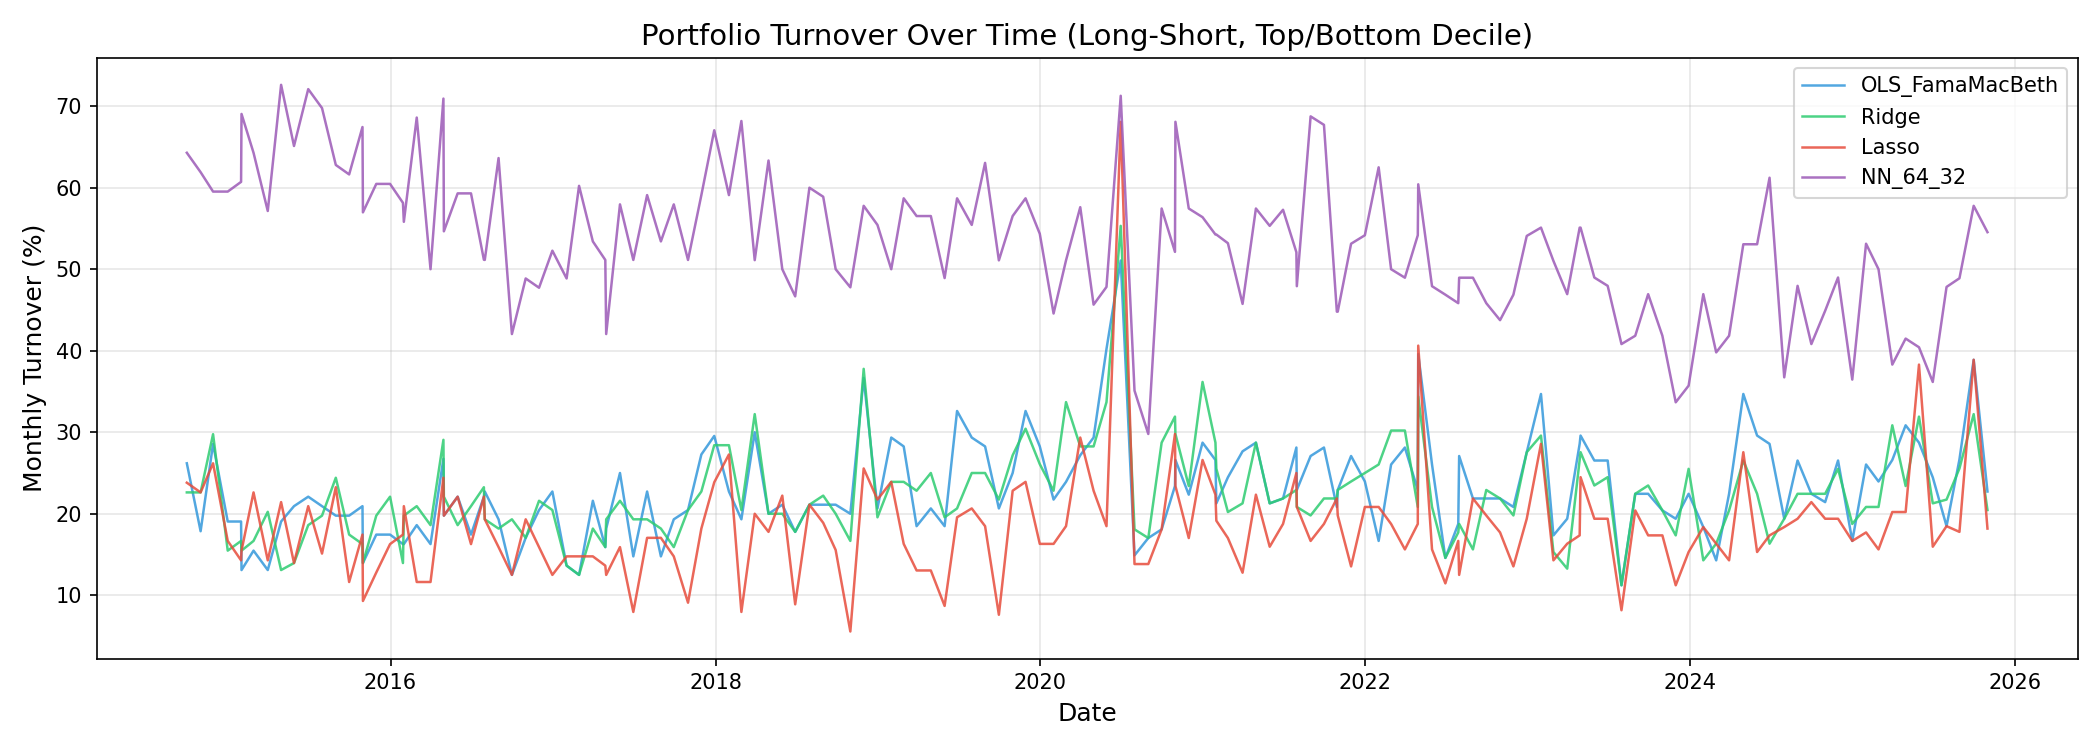
\includegraphics[width=0.8\textwidth]{turnover_timeseries.png}
    \caption{Monthly portfolio turnover for each model over the evaluation period.}
    \label{fig:turnover_ts}
\end{figure}

\begin{figure}[H]
    \centering
    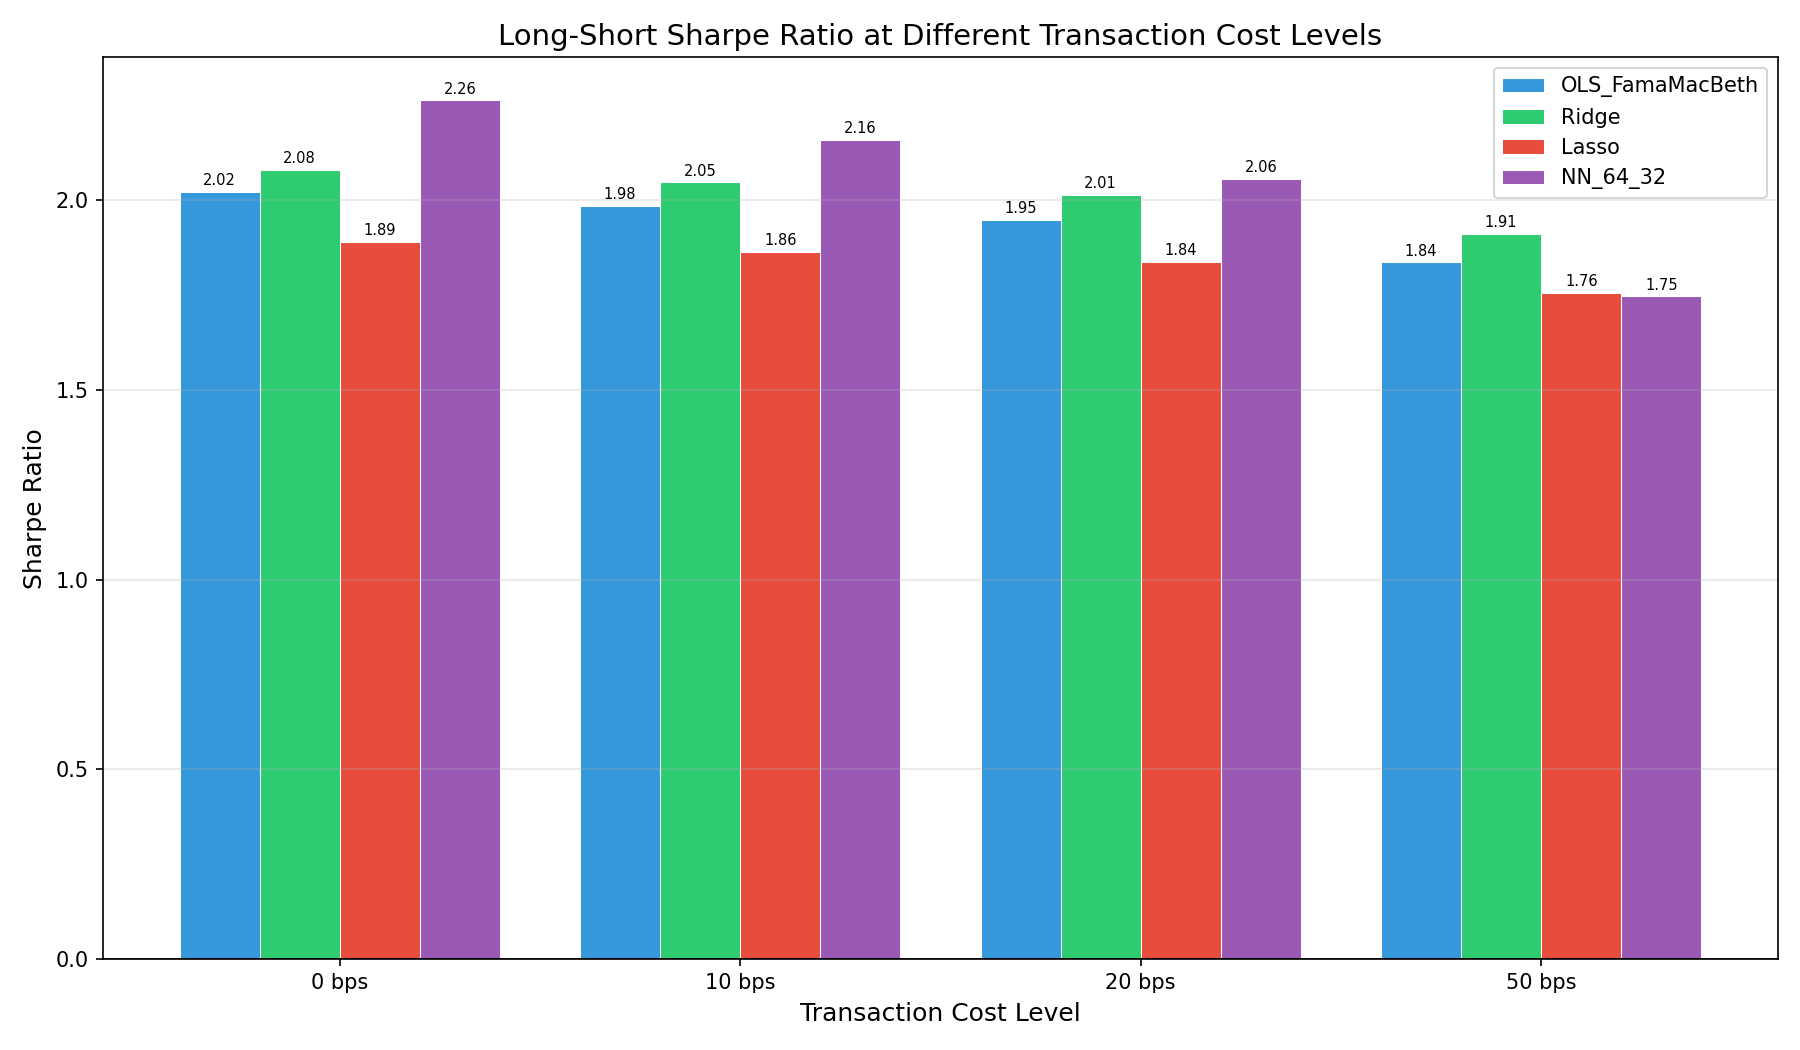
\includegraphics[width=0.7\textwidth]{sharpe_after_costs.png}
    \caption{Sharpe ratio as a function of transaction cost level for each model.}
    \label{fig:sharpe_costs}
\end{figure}

% ------------------------------------------------------------
\subsection{Feature Importance}
\label{sec:feature_importance}
% ------------------------------------------------------------

We compare feature importance across three methods: Fama--MacBeth absolute $t$-statistics, Lasso surviving coefficient magnitudes, and neural network permutation importance \cite{breiman2001}. All importance measures are normalized to $[0, 1]$ for comparability. The results are shown in Figure~\ref{fig:importance_comparison}.

\begin{figure}[H]
    \centering
    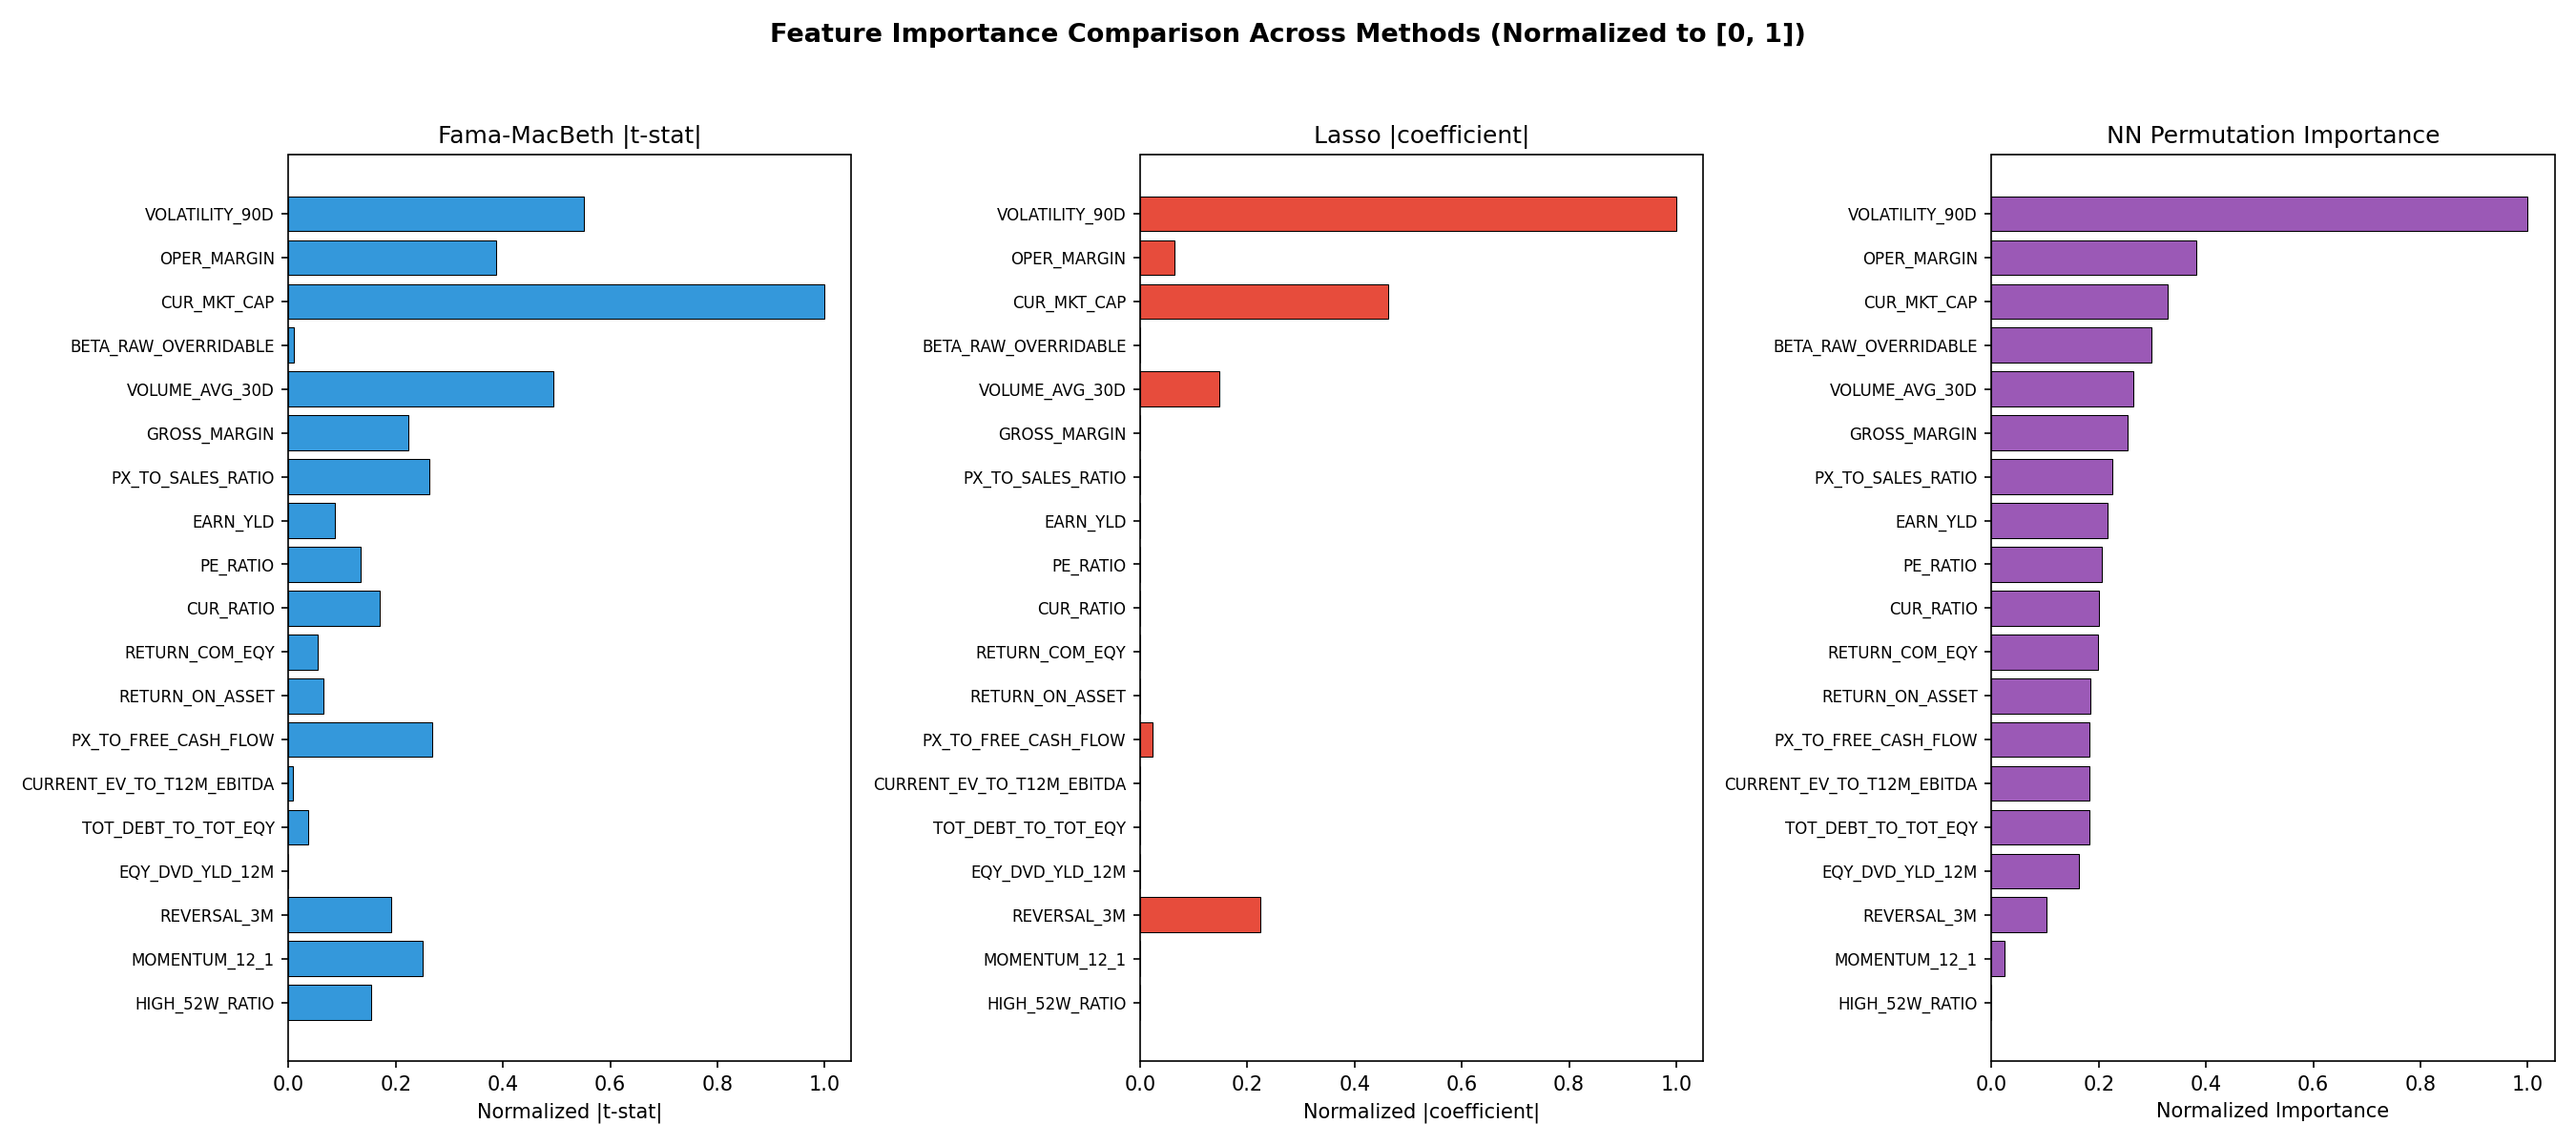
\includegraphics[width=\textwidth]{feature_importance_comparison.png}
    \caption{Normalized feature importance across three methods: Fama--MacBeth $|t|$-statistics (left), Lasso $|\text{coefficient}|$ (center), and neural network permutation importance (right).}
    \label{fig:importance_comparison}
\end{figure}

The strongest consensus finding is that \textbf{90-day realized volatility} (\verb|VOLATILITY_90D|) is the most important feature. It is ranked first by both Lasso (normalized importance 1.00) and the neural network (1.00), and second by Fama--MacBeth (0.55). \textbf{Market capitalization} is the strongest Fama--MacBeth factor (1.00) and ranks second for Lasso (0.46) and third for the NN (0.33). \textbf{Operating margin} is consistently important across all three methods.

A notable difference is that the NN assigns substantial importance to features that Lasso zeroes out entirely, including \verb|BETA_RAW_OVERRIDABLE| (NN: 0.30, Lasso: 0.00), \verb|GROSS_MARGIN| (NN: 0.25, Lasso: 0.00), and \verb|EARN_YLD| (NN: 0.22, Lasso: 0.00). This suggests the NN is exploiting nonlinear interactions among these features that a linear model cannot capture.

\begin{figure}[H]
    \centering
    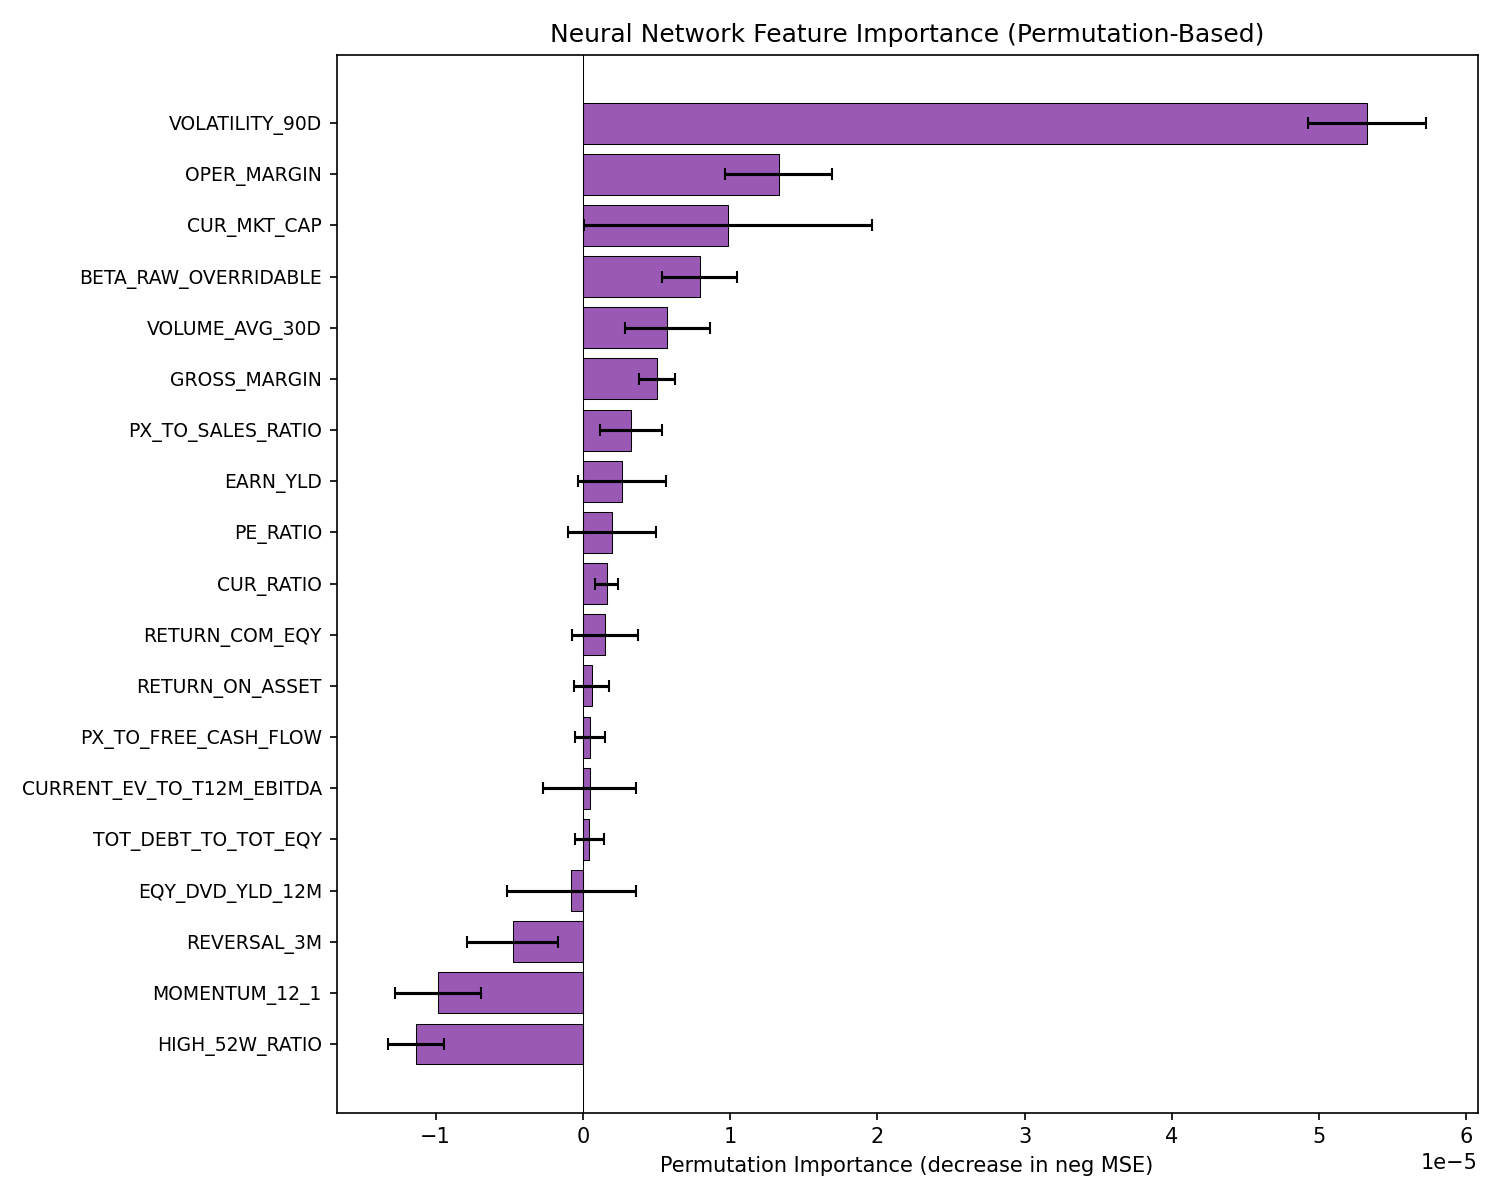
\includegraphics[width=0.8\textwidth]{nn_feature_importance.png}
    \caption{Neural network permutation importance for all 19 features. VOLATILITY\_90D dominates.}
    \label{fig:nn_importance}
\end{figure}

% ------------------------------------------------------------
\subsection{Fama--French Factor Attribution}
\label{sec:ff_alpha}
% ------------------------------------------------------------

To determine whether the portfolio returns are compensation for exposure to known risk factors or represent genuine alpha, we regress each model's monthly long-short returns on the Fama--French five factors \cite{fama2015} plus momentum \cite{carhart1997}:

\begin{equation}
    R_{p,t} - R_{f,t} = \alpha + \beta_1 \text{MKT-RF}_t + \beta_2 \text{SMB}_t + \beta_3 \text{HML}_t + \beta_4 \text{RMW}_t + \beta_5 \text{CMA}_t + \beta_6 \text{UMD}_t + \varepsilon_t
\end{equation}

The results are reported in Table~\ref{tab:ff_alpha}.

\begin{table}[H]
\centering
\caption{Fama--French 5-factor + momentum regression. All alphas are annualized and significant at the 1\% level.}
\label{tab:ff_alpha}
\begin{tabular}{lcccccccc}
\toprule
Model & $\alpha$ (ann.) & $t_\alpha$ & $R^2$ & MKT-RF & SMB & HML & RMW & CMA \\
\midrule
FM    & 28.53\% & 7.02 & 0.115 & $-0.02$ & $+0.33$ & $-0.45$ & $+0.25$ & $+0.65$ \\
Ridge & 30.90\% & 7.23 & 0.111 & $-0.03$ & $+0.32$ & $-0.49$ & $+0.22$ & $+0.68$ \\
Lasso & 28.88\% & 6.51 & 0.096 & $-0.03$ & $+0.36$ & $-0.48$ & $+0.23$ & $+0.60$ \\
NN    & 27.90\% & \textbf{7.75} & \textbf{0.086} & $-0.02$ & $+0.30$ & $-0.38$ & $+0.20$ & $+0.40$ \\
\bottomrule
\end{tabular}
\end{table}

All four models generate highly significant alpha ($t > 6.5$, $p < 0.001$) after controlling for six standard risk factors. The annualized alphas range from 27.90\% (NN) to 30.90\% (Ridge). Critically, the low $R^2$ values (8.6\%--11.5\%) indicate that known factors explain only a small fraction of the portfolio returns, meaning the strategies are capturing genuinely novel signal rather than repackaging known factor exposures.

The factor loadings are consistent across models: all portfolios load positively on SMB (small-cap tilt), negatively on HML (anti-value or growth tilt), and positively on CMA (conservative investment tilt). Near-zero market beta confirms that the long-short construction effectively hedges market risk. The neural network has the lowest $R^2$ (0.086) and the smallest factor loadings, suggesting that its signal is the most distinct from traditional risk factors.

\begin{figure}[H]
    \centering
    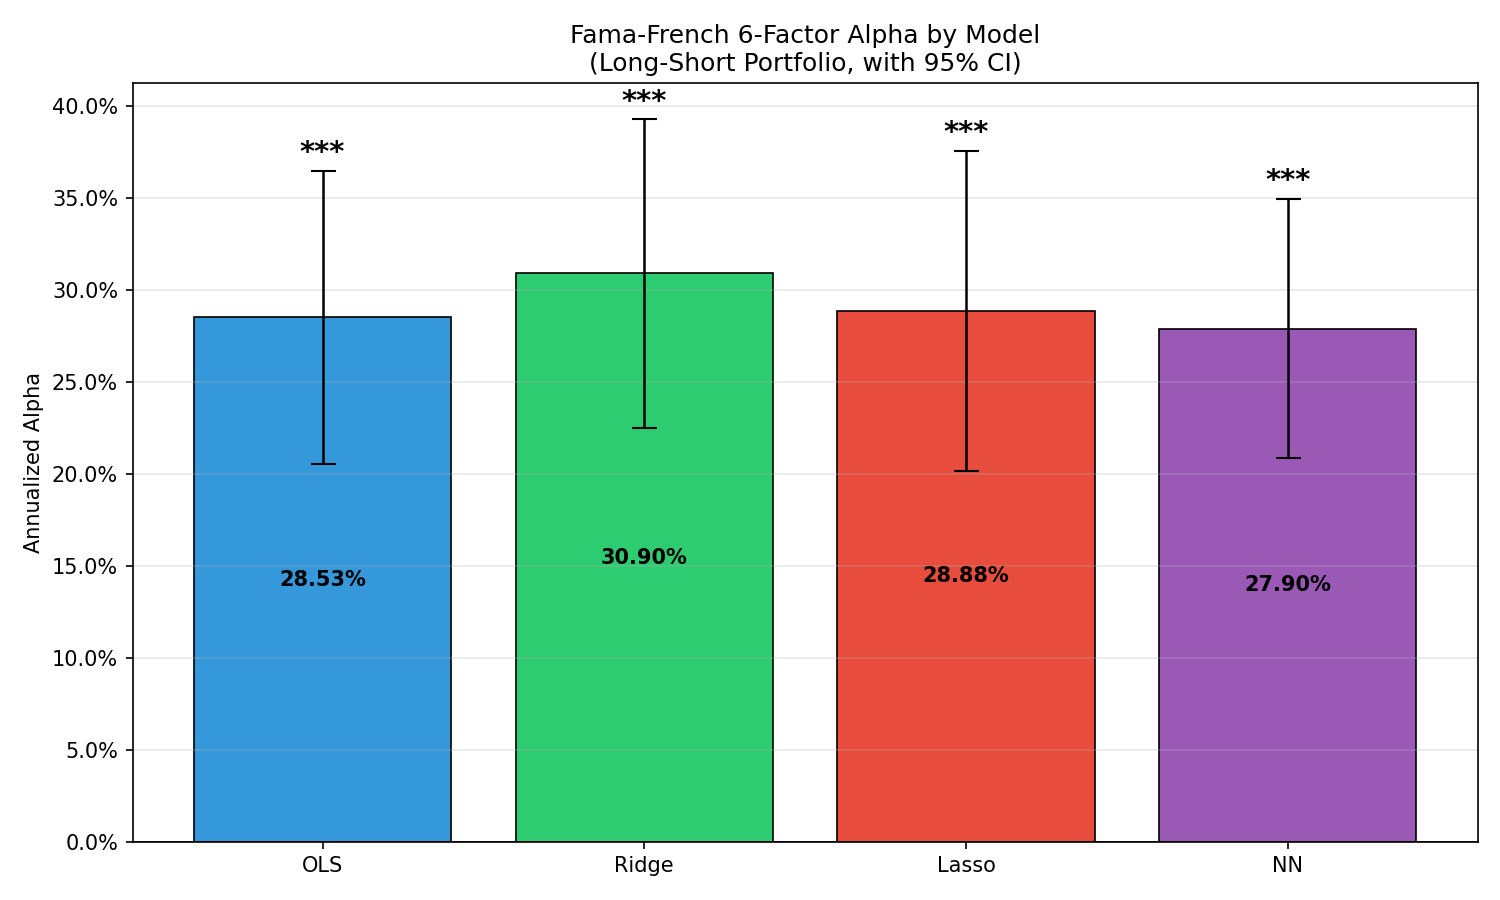
\includegraphics[width=0.7\textwidth]{alpha_comparison.png}
    \caption{Annualized Fama--French alpha by model. All alphas are significant at the 1\% level (***).}
    \label{fig:alpha}
\end{figure}

% ============================================================
\section{Division of Labor}
\label{sec:division}
% ============================================================

% TODO: Describe how the work was divided among team members.

% ============================================================
\section{Conclusion}
\label{sec:conclusion}
% ============================================================

We have presented a comprehensive study of cross-sectional stock return prediction using six machine learning methods, all implemented as distributed PySpark pipelines and evaluated under a rigorous expanding-window framework on a panel of 93{,}237 S\&P 500 stock-month observations.

Our main findings are as follows:

\begin{enumerate}
    \item \textbf{Ridge regression is the strongest point predictor.} It achieves the highest mean IC (0.0623), the highest raw annualized return (30.90\%), and the highest cost-adjusted Sharpe ratio at realistic transaction cost levels (1.91 at 50 bps). Its advantage over the unregularized Fama--MacBeth baseline confirms the value of regularization for this task.

    \item \textbf{The neural network delivers the best risk-adjusted performance.} Despite a slightly lower IC (0.0577), the NN\_64\_32 model achieves the highest Sharpe ratio (2.27), the lowest maximum drawdown ($-5.76\%$), and the highest hit rate (73.65\%). Its crash resilience is remarkable: during the three crash months in our sample, the NN portfolio generated $+45\%$ annualized returns while linear models lost over 30\%.

    \item \textbf{All models generate significant alpha.} After controlling for the Fama--French five factors and momentum, all four models produce annualized alpha exceeding 27\% with $t$-statistics above 6.5. The low factor model $R^2$ (below 12\%) confirms that the strategies capture signal beyond traditional risk factor exposures. The NN's returns are the least explained by known factors ($R^2 = 8.6\%$).

    \item \textbf{Turnover is the neural network's Achilles heel.} The NN's monthly turnover (53\%) is $2.4\times$ that of Ridge, causing its Sharpe advantage to disappear at transaction costs above approximately 30 bps. This highlights turnover-aware optimization as a critical direction for neural network-based strategies.

    \item \textbf{Parallelization benefits scale with per-task complexity.} The NN achieves $4.37\times$ speedup at 16 cores, while lightweight models like Fama--MacBeth barely benefit ($1.10\times$). This pattern is consistent with Amdahl's law: the communication overhead of distributed Spark execution is amortized only when individual tasks are sufficiently compute-intensive.

    \item \textbf{Volatility is the dominant cross-sectional predictor.} 90-day realized volatility is the most important feature for both Lasso and the neural network, and the second most important for Fama--MacBeth. This finding is robust across all three importance methods and suggests that the low-volatility anomaly (in its cross-sectional form) remains a powerful source of return predictability.
\end{enumerate}

Several limitations merit acknowledgment. Our analysis covers only U.S.\ large-cap equities (S\&P 500), and the results may not generalize to international markets or smaller-capitalization universes. The crash regime comprises only three months, limiting the statistical power of regime-conditional conclusions. We do not optimize portfolio construction for turnover constraints, which could substantially improve the NN's cost-adjusted performance. Finally, our neural network architecture search is limited to three depth configurations; more extensive hyperparameter optimization could yield further gains.

% ============================================================
\bibliographystyle{plain}
\begin{thebibliography}{10}

\bibitem{fama1973}
E.~F. Fama and J.~D. MacBeth,
``Risk, Return, and Equilibrium: Empirical Tests,''
\textit{The Journal of Political Economy}, Vol.~81, No.~3, pp.~607--636, 1973.

\bibitem{hoerl1970}
A.~E. Hoerl and R.~W. Kennard,
``Ridge Regression: Biased Estimation for Nonorthogonal Problems,''
\textit{Technometrics}, Vol.~12, No.~1, pp.~55--67, 1970.

\bibitem{tibshirani1996}
R.~Tibshirani,
``Regression Shrinkage and Selection via the Lasso,''
\textit{Journal of the Royal Statistical Society: Series B}, Vol.~58, No.~1, pp.~267--288, 1996.

\bibitem{fama2015}
E.~F. Fama and K.~R. French,
``A Five-Factor Asset Pricing Model,''
\textit{Journal of Financial Economics}, Vol.~116, No.~1, pp.~1--22, 2015.

\bibitem{carhart1997}
M.~M. Carhart,
``On Persistence in Mutual Fund Performance,''
\textit{The Journal of Finance}, Vol.~52, No.~1, pp.~57--82, 1997.

\bibitem{gu2020}
S.~Gu, B.~Kelly, and D.~Xiu,
``Empirical Asset Pricing via Machine Learning,''
\textit{The Review of Financial Studies}, Vol.~33, No.~5, pp.~2223--2273, 2020.

\bibitem{diebold1995}
F.~X. Diebold and R.~S. Mariano,
``Comparing Predictive Accuracy,''
\textit{Journal of Business \& Economic Statistics}, Vol.~13, No.~3, pp.~253--263, 1995.

\bibitem{breiman2001}
L.~Breiman,
``Random Forests,''
\textit{Machine Learning}, Vol.~45, No.~1, pp.~5--32, 2001.

\bibitem{bottou2010}
L.~Bottou,
``Large-Scale Machine Learning with Stochastic Gradient Descent,''
\textit{Proceedings of COMPSTAT}, pp.~177--186, 2010.

\bibitem{dean2012}
J.~Dean, G.~Corrado, R.~Monga, K.~Chen, M.~Devin, Q.~Le, M.~Mao, M.~Ranzato, A.~Senior, P.~Tucker, K.~Yang, and A.~Ng,
``Large Scale Distributed Deep Networks,''
\textit{Advances in Neural Information Processing Systems}, Vol.~25, 2012.

\end{thebibliography}

\end{document}
